\documentclass[12pt,a4paper,]{book}
\def\ifdoblecara{} %% set to true
\def\ifprincipal{} %% set to true
\let\ifprincipal\undefined %% set to false
\def\ifcitapandoc{} %% set to true
\let\ifcitapandoc\undefined %% set to false
\usepackage{lmodern}
\usepackage{amssymb,amsmath}
\usepackage{ifxetex,ifluatex}
%\usepackage{fixltx2e} % provides \textsubscript %PLLC
\ifnum 0\ifxetex 1\fi\ifluatex 1\fi=0 % if pdftex
  \usepackage[T1]{fontenc}
  \usepackage[utf8]{inputenc}
\else % if luatex or xelatex
  \ifxetex
    \usepackage{mathspec}
  \else
    \usepackage{fontspec}
  \fi
  \defaultfontfeatures{Ligatures=TeX,Scale=MatchLowercase}
\fi
% use upquote if available, for straight quotes in verbatim environments
\IfFileExists{upquote.sty}{\usepackage{upquote}}{}
% use microtype if available
\IfFileExists{microtype.sty}{%
\usepackage{microtype}
\UseMicrotypeSet[protrusion]{basicmath} % disable protrusion for tt fonts
}{}
\usepackage[margin = 2.5cm]{geometry}
\usepackage{hyperref}
\hypersetup{unicode=true,
            pdfauthor={Nombre Completo Autor},
              pdfborder={0 0 0},
              breaklinks=true}
\urlstyle{same}  % don't use monospace font for urls
\usepackage{natbib}
\bibliographystyle{plainnat}
%%% desaptivado lo que sigue
%\usepackage[usenames,dvipsnames]{xcolor}  %new PLLC
\IfFileExists{parskip.sty}{%
\usepackage{parskip}
}{% else
\setlength{\parindent}{0pt}
\setlength{\parskip}{6pt plus 2pt minus 1pt}
}
\setlength{\emergencystretch}{3em}  % prevent overfull lines
\providecommand{\tightlist}{%
  \setlength{\itemsep}{0pt}\setlength{\parskip}{0pt}}
\setcounter{secnumdepth}{5}
% Redefines (sub)paragraphs to behave more like sections
\ifx\paragraph\undefined\else
\let\oldparagraph\paragraph
\renewcommand{\paragraph}[1]{\oldparagraph{#1}\mbox{}}
\fi
\ifx\subparagraph\undefined\else
\let\oldsubparagraph\subparagraph
\renewcommand{\subparagraph}[1]{\oldsubparagraph{#1}\mbox{}}
\fi

%%% Use protect on footnotes to avoid problems with footnotes in titles
\let\rmarkdownfootnote\footnote%
\def\footnote{\protect\rmarkdownfootnote}


  \title{}
    \author{Nombre Completo Autor}
      \date{06/02/2024}


%%%%%%% inicio: latex_preambulo.tex PLLC

%% UTILIZA CODIFICACIÓN UTF-8
%% MODIFICARLO CONVENIENTEMENTE PARA USARLO CON OTRAS CODIFICACIONES


%\usepackage[spanish,es-nodecimaldot,es-noshorthands]{babel}
\usepackage[spanish,es-nodecimaldot,es-noshorthands,es-tabla]{babel}
% Ver: es-tabla (en: https://osl.ugr.es/CTAN/macros/latex/contrib/babel-contrib/spanish/spanish.pdf)
% es-tabla (en: https://tex.stackexchange.com/questions/80443/change-the-word-table-in-table-captions)
\usepackage{float}
\usepackage{placeins}
\usepackage{fancyhdr}   %desaptivado por mí
% Solucion: ! LaTeX Error: Command \counterwithout already defined.
% https://tex.stackexchange.com/questions/425600/latex-error-command-counterwithout-already-defined
\let\counterwithout\relax
\let\counterwithin\relax
\usepackage{chngcntr}
%\usepackage{microtype}  %antes en template PLLC
\usepackage[utf8]{inputenc}
\usepackage[T1]{fontenc} % Usa codificación 8-bit que tiene 256 glyphs

%\usepackage[dvipsnames]{xcolor}
%\usepackage[usenames,dvipsnames]{xcolor}  %new
\usepackage{pdfpages}
%\usepackage{natbib}




% Para portada: latex_paginatitulo_mod_ST02.tex (inicio)
\usepackage{tikz}
\usepackage{epigraph}
\renewcommand\epigraphflush{flushright}
\renewcommand\epigraphsize{\normalsize}
\setlength\epigraphwidth{0.7\textwidth}

\definecolor{titlepagecolor}{cmyk}{1,.60,0,.40}

%\DeclareFixedFont{\titlefont}{T1}{ppl}{b}{it}{0.5in}

% \makeatletter
% \def\printauthor{%
%     {\large \@author}}
% \makeatother
% \author{%
%     Author 1 name \\
%     Department name \\
%     \texttt{email1@example.com}\vspace{20pt} \\
%     Author 2 name \\
%     Department name \\
%     \texttt{email2@example.com}
%     }

% The following code is borrowed from: https://tex.stackexchange.com/a/86310/10898

\newcommand\titlepagedecoration{%
\begin{tikzpicture}[remember picture,overlay,shorten >= -10pt]

\coordinate (aux1) at ([yshift=-15pt]current page.north east);
\coordinate (aux2) at ([yshift=-410pt]current page.north east);
\coordinate (aux3) at ([xshift=-4.5cm]current page.north east);
\coordinate (aux4) at ([yshift=-150pt]current page.north east);

\begin{scope}[titlepagecolor!40,line width=12pt,rounded corners=12pt]
\draw
  (aux1) -- coordinate (a)
  ++(225:5) --
  ++(-45:5.1) coordinate (b);
\draw[shorten <= -10pt]
  (aux3) --
  (a) --
  (aux1);
\draw[opacity=0.6,titlepagecolor,shorten <= -10pt]
  (b) --
  ++(225:2.2) --
  ++(-45:2.2);
\end{scope}
\draw[titlepagecolor,line width=8pt,rounded corners=8pt,shorten <= -10pt]
  (aux4) --
  ++(225:0.8) --
  ++(-45:0.8);
\begin{scope}[titlepagecolor!70,line width=6pt,rounded corners=8pt]
\draw[shorten <= -10pt]
  (aux2) --
  ++(225:3) coordinate[pos=0.45] (c) --
  ++(-45:3.1);
\draw
  (aux2) --
  (c) --
  ++(135:2.5) --
  ++(45:2.5) --
  ++(-45:2.5) coordinate[pos=0.3] (d);   
\draw 
  (d) -- +(45:1);
\end{scope}
\end{tikzpicture}%
}

% Para portada: latex_paginatitulo_mod_ST02.tex (fin)

% Para portada: latex_paginatitulo_mod_OV01.tex (inicio)
\usepackage{cpimod}
% Para portada: latex_paginatitulo_mod_OV01.tex (fin)

% Para portada: latex_paginatitulo_mod_OV03.tex (inicio)
\usepackage{KTHEEtitlepage}
% Para portada: latex_paginatitulo_mod_OV03.tex (fin)

\renewcommand{\contentsname}{Índice}
\renewcommand{\listfigurename}{Índice de figuras}
\renewcommand{\listtablename}{Índice de tablas}
\newcommand{\bcols}{}
\newcommand{\ecols}{}
\newcommand{\bcol}[1]{\begin{minipage}{#1\linewidth}}
\newcommand{\ecol}{\end{minipage}}
\newcommand{\balertblock}[1]{\begin{alertblock}{#1}}
\newcommand{\ealertblock}{\end{alertblock}}
\newcommand{\bitemize}{\begin{itemize}}
\newcommand{\eitemize}{\end{itemize}}
\newcommand{\benumerate}{\begin{enumerate}}
\newcommand{\eenumerate}{\end{enumerate}}
\newcommand{\saltopagina}{\newpage}
\newcommand{\bcenter}{\begin{center}}
\newcommand{\ecenter}{\end{center}}
\newcommand{\beproof}{\begin{proof}} %new
\newcommand{\eeproof}{\end{proof}} %new
%De: https://texblog.org/2007/11/07/headerfooter-in-latex-with-fancyhdr/
% \fancyhead
% E: Even page
% O: Odd page
% L: Left field
% C: Center field
% R: Right field
% H: Header
% F: Footer
%\fancyhead[CO,CE]{Resultados}

%OPCION 1
% \fancyhead[LE,RO]{\slshape \rightmark}
% \fancyhead[LO,RE]{\slshape \leftmark}
% \fancyfoot[C]{\thepage}
% \renewcommand{\headrulewidth}{0.4pt}
% \renewcommand{\footrulewidth}{0pt}

%OPCION 2
% \fancyhead[LE,RO]{\slshape \rightmark}
% \fancyfoot[LO,RE]{\slshape \leftmark}
% \fancyfoot[LE,RO]{\thepage}
% \renewcommand{\headrulewidth}{0.4pt}
% \renewcommand{\footrulewidth}{0.4pt}
%%%%%%%%%%
\usepackage{calc,amsfonts}
% Elimina la cabecera de páginas impares vacías al finalizar los capítulos
\usepackage{emptypage}
\makeatletter

\definecolor{ocre}{RGB}{25,25,243} % Define el color naranja usado para resaltar algunas salidas

%\usepackage{calc} 

\usepackage{lipsum}

%\usepackage{tikz} % Requerido para dibujar formas personalizadas

%\usepackage{amsmath,amsthm,amssymb,amsfonts}
\usepackage{amsthm}

%%%%%%% DE TEOREMAS %%%%%%%%%%
% Boxed/framed environments
\newtheoremstyle{ocrenumbox}% % Theorem style name
{0pt}% Space above
{0pt}% Space below
{\normalfont}% % Body font
{}% Indent amount
%%% Descomentado por mí , letra bf: de teoremas,def,ejemplos
{\small\bf\sffamily\color{ocre}}% % Theorem head font
{\;}% Punctuation after theorem head
{0.25em}% Space after theorem head
{\small\sffamily\color{ocre}\thmname{#1}\nobreakspace\thmnumber{\@ifnotempty{#1}{}\@upn{#2}}% Theorem text (e.g. Theorem 2.1)
%%%% \bfseries: bf para textos de: teoremas,definiciones, ejemplos
\thmnote{\nobreakspace\the\thm@notefont\sffamily\bfseries\color{black}---\nobreakspace#3.}} % Optional theorem note
\renewcommand{\qedsymbol}{$\blacksquare$}% Optional qed square

\newtheoremstyle{blacknumex}% Theorem style name
{5pt}% Space above
{5pt}% Space below
{\normalfont}% Body font
%{\textit}% Body font
{} % Indent amount
%%% Descomentado por mí 
%{\small\bf\sffamily}% Theorem head font
{\small\bf\sffamily}% Theorem head font
{\;}% Punctuation after theorem head
{0.25em}% Space after theorem head
{\small\sffamily{\tiny\ensuremath{\blacksquare}}\nobreakspace\thmname{#1}\nobreakspace\thmnumber{\@ifnotempty{#1}{}\@upn{#2}}% Theorem text (e.g. Theorem 2.1)
\thmnote{\nobreakspace\the\thm@notefont\sffamily\bfseries---\nobreakspace#3.}}% Optional theorem note

\newtheoremstyle{blacknumbox} % Theorem style name
{0pt}% Space above
{0pt}% Space below
{\normalfont}% Body font
%{\textit}% Body font
{}% Indent amount
%%% Descomentado por mí 
%{\small\bf\sffamily}% Theorem head font
{\small\bf\sffamily}% Theorem head font
{\;}% Punctuation after theorem head
{0.25em}% Space after theorem head
{\small\sffamily\thmname{#1}\nobreakspace\thmnumber{\@ifnotempty{#1}{}\@upn{#2}}% Theorem text (e.g. Theorem 2.1)
\thmnote{\nobreakspace\the\thm@notefont\sffamily\bfseries---\nobreakspace#3.}}% Optional theorem note

% Non-boxed/non-framed environments
\newtheoremstyle{ocrenum}% % Theorem style name
{5pt}% Space above
{5pt}% Space below
{\normalfont}% % Body font
%{\textit}% Body font
{}% Indent amount
%%% Descomentado por mí 
%{\small\bf\sffamily\color{ocre}}% % Theorem head font
{\small\bf\sffamily\color{ocre}}% % Theorem head font
{\;}% Punctuation after theorem head
{0.25em}% Space after theorem head
{\small\sffamily\color{ocre}\thmname{#1}\nobreakspace\thmnumber{\@ifnotempty{#1}{}\@upn{#2}}% Theorem text (e.g. Theorem 2.1)
\thmnote{\nobreakspace\the\thm@notefont\sffamily\bfseries\color{black}---\nobreakspace#3.}} % Optional theorem note
\renewcommand{\qedsymbol}{$\blacksquare$}% Optional qed square
\makeatother


% Define el estilo del texto theorem para cada tipo definido anteriormente
\newcounter{dummy} 
\numberwithin{dummy}{section}
\theoremstyle{ocrenumbox}

\newtheorem{theoremeT}[dummy]{Teorema}  % (Pedro: Theorem)

\newtheorem{problem}{Problema}[chapter]  % (Pedro: Problem)

\newtheorem{exerciseT}{Ejercicio}[chapter] % (Pedro: Exercise)

%%%%%%%%%%% color texto ejemplos
\theoremstyle{ocrenumbox}
\newtheorem{exampleT}{Ejemplo}[chapter] % (Pedro: Example)

\theoremstyle{ocrenumbox}

\newtheorem{vocabulary}{Vocabulario}[chapter]  % (Pedro: Vocabulary)

\newtheorem{definitionT}{Definición}[section]  % (Pedro: Definition)
\newtheorem{corollaryT}[dummy]{Corolario}  % (Pedro: Corollary)
\theoremstyle{ocrenumbox}
\newtheorem{proposition}[dummy]{Proposición} % (Pedro: Proposition)

\usepackage[framemethod=default]{mdframed}


\newcommand{\intoo}[2]{\mathopen{]}#1\,;#2\mathclose{[}}
\newcommand{\ud}{\mathop{\mathrm{{}d}}\mathopen{}}
\newcommand{\intff}[2]{\mathopen{[}#1\,;#2\mathclose{]}}
\newtheorem{notation}{Notation}[chapter]


%\mdfdefinestyle{exampledefault}{%
%rightline=true,innerleftmargin=10,innerrightmargin=10,
%frametitlerule=true,frametitlerulecolor=green,
%frametitlebackgroundcolor=yellow,
%frametitlerulewidth=2pt}


% Theorem box
\newmdenv[skipabove=7pt,
skipbelow=7pt,
%backgroundcolor=black!5,
rightline=false,
leftline=false,
topline=false,
bottomline=false,
linecolor=gray,
%backgroundcolor=black!5,
innerleftmargin=5pt,
innerrightmargin=5pt,
innertopmargin=10pt,%5pt
leftmargin=0cm,
rightmargin=0cm,
linewidth=0pt,
innerbottommargin=0pt]{tBox}

% Exercise box	  
\newmdenv[skipabove=7pt,
skipbelow=7pt,
rightline=false,
leftline=true,
topline=false,
bottomline=false,
backgroundcolor=ocre!10,
linecolor=ocre,
innerleftmargin=5pt,
innerrightmargin=5pt,
innertopmargin=10pt,%5pt
innerbottommargin=5pt,
leftmargin=0cm,
rightmargin=0cm,
linewidth=4pt]{eBox}	

% Definition box
\newmdenv[skipabove=7pt,
skipbelow=7pt,
rightline=false,
leftline=false,
topline=false,
bottomline=false,
%backgroundcolor=black!5,
linecolor=gray,
innerleftmargin=5pt,
innerrightmargin=5pt,
innertopmargin=10pt,%0pt
leftmargin=0cm,
rightmargin=0cm,
linewidth=0pt,
innerbottommargin=0pt]{dBox}	

% Corollary box
\newmdenv[skipabove=7pt,
skipbelow=7pt,
rightline=false,
leftline=true,
topline=false,
bottomline=false,
linecolor=gray,
backgroundcolor=black!5,
innerleftmargin=5pt,
innerrightmargin=5pt,
innertopmargin=10pt,%5pt
leftmargin=0cm,
rightmargin=0cm,
linewidth=5pt,
innerbottommargin=5pt]{cBox}

%%% nuevo ejemplo
% example box
\newmdenv[skipabove=7pt,
skipbelow=7pt,
rightline=false,
leftline=false,
topline=false,
bottomline=false,
%backgroundcolor=black!5,
linecolor=gray,
innerleftmargin=5pt,
innerrightmargin=5pt,
innertopmargin=10pt,%0pt
leftmargin=0cm,
rightmargin=0cm,
linewidth=0pt,
innerbottommargin=0pt]{exBox}	



% Crea un entorno para cada tipo de theorem y le asigna un estilo 
% con ayuda de las cajas coloreadas anteriores

%\newenvironment{theorem}{\begin{tBox}\begin{theoremeT}}{\end{theoremeT}\end{tBox}}

\newenvironment{exercise}{\begin{eBox}\begin{exerciseT}}{\hfill{\color{ocre}\tiny\ensuremath{\blacksquare}}\end{exerciseT}\end{eBox}}				  
%\newenvironment{definition}{\begin{dBox}\begin{definitionT}}{\end{definitionT}\end{dBox}}	

%%%% Cuadrado negro al final de: teorema, definicion, ejemplos

\newenvironment{theorem}{\begin{theoremeT}}{\hfill{\small\ensuremath{\blacksquare}}\end{theoremeT}}		

\newenvironment{example}{\begin{exampleT}}{\hfill{\small\ensuremath{\blacksquare}}\end{exampleT}}		

\newenvironment{definition}{\begin{definitionT}}{\hfill{\small\ensuremath{\blacksquare}}\end{definitionT}}		


%%%%%% nuevo ejemplo
%\newenvironment{example}{\begin{exBox}\begin{exampleT}}{\end{exampleT}\end{exBox}}	

\newenvironment{corollary}{\begin{cBox}\begin{corollaryT}}{\end{corollaryT}\end{cBox}}	

%	ENVIRONMENT remark
\newenvironment{remark}{\par\vspace{10pt}\small 
% Espacio blanco vertical sobre la nota y tamaño de fuente menor
\begin{list}{}{
\leftmargin=35pt % Indentación sobre la izquierda
\rightmargin=25pt}\item\ignorespaces % Indentación sobre la derecha
\makebox[-2.5pt]{\begin{tikzpicture}[overlay]
\node[draw=ocre!60,line width=1pt,circle,fill=ocre!25,font=\sffamily\bfseries,inner sep=2pt,outer sep=0pt] at (-15pt,0pt){\textcolor{ocre}{N}}; \end{tikzpicture}} % R naranja en un círculo (Pedro)
\advance\baselineskip -1pt}{\end{list}\vskip5pt} 
% Espaciado de línea más estrecho y espacio en blanco después del comentario


\newenvironment{solutionExe}{\par\vspace{10pt}\small 
\begin{list}{}{
\leftmargin=35pt 
\rightmargin=25pt}\item\ignorespaces 
\makebox[-2.5pt]{\begin{tikzpicture}[overlay]
\node[draw=ocre!60,line width=1pt,circle,fill=ocre!25,font=\sffamily\bfseries,inner sep=2pt,outer sep=0pt] at (-15pt,0pt){\textcolor{ocre}{S}}; \end{tikzpicture}} 
\advance\baselineskip -1pt}{\end{list}\vskip5pt} 

\newenvironment{solutionExa}{\par\vspace{10pt}\small 
\begin{list}{}{
\leftmargin=35pt 
\rightmargin=25pt}\item\ignorespaces 
\makebox[-2.5pt]{\begin{tikzpicture}[overlay]
\node[draw=ocre!60,line width=1pt,circle,fill=ocre!55,font=\sffamily\bfseries,inner sep=2pt,outer sep=0pt] at (-15pt,0pt){\textcolor{ocre}{S}}; \end{tikzpicture}} 
\advance\baselineskip -1pt}{\end{list}\vskip5pt} 

\usepackage{tcolorbox}

\usetikzlibrary{trees}

\theoremstyle{ocrenum}
\newtheorem{solutionT}[dummy]{Solución}  % (Pedro: Corollary)
\newenvironment{solution}{\begin{cBox}\begin{solutionT}}{\end{solutionT}\end{cBox}}	


\newcommand{\tcolorboxsolucion}[2]{%
\begin{tcolorbox}[colback=green!5!white,colframe=green!75!black,title=#1] 
 #2
 %\tcblower  % pone una línea discontinua
\end{tcolorbox}
}% final definición comando

\newtcbox{\mybox}[1][green]{on line,
arc=0pt,outer arc=0pt,colback=#1!10!white,colframe=#1!50!black, boxsep=0pt,left=1pt,right=1pt,top=2pt,bottom=2pt, boxrule=0pt,bottomrule=1pt,toprule=1pt}


%\mdfdefinestyle{exampledefault}{%
%rightline=true,innerleftmargin=10,innerrightmargin=10,
%frametitlerule=true,frametitlerulecolor=green,
%frametitlebackgroundcolor=yellow,
%frametitlerulewidth=2pt}



\newcommand{\betheorem}{\begin{theorem}}
\newcommand{\eetheorem}{\end{theorem}}

\newcommand{\bedefinition}{\begin{definition}}
\newcommand{\eedefinition}{\end{definition}}

\newcommand{\beremark}{\begin{remark}}
\newcommand{\eeremark}{\end{remark}}

\newcommand{\beexercise}{\begin{exercise}}
\newcommand{\eeexercise}{\end{exercise}}

\newcommand{\beexample}{\begin{example}}
\newcommand{\eeexample}{\end{example}}

\newcommand{\becorollary}{\begin{corollary}}
\newcommand{\eecorollary}{\end{corollary}}


\newcommand{\besolutionExe}{\begin{solutionExe}}
\newcommand{\eesolutionExe}{\end{solutionExe}}

\newcommand{\besolutionExa}{\begin{solutionExa}}
\newcommand{\eesolutionExa}{\end{solutionExa}}


%%%%%%%%


% Caja Salida Markdown
\newmdenv[skipabove=7pt,
skipbelow=7pt,
rightline=false,
leftline=true,
topline=false,
bottomline=false,
backgroundcolor=GreenYellow!10,
linecolor=GreenYellow!80,
innerleftmargin=5pt,
innerrightmargin=5pt,
innertopmargin=10pt,%5pt
innerbottommargin=5pt,
leftmargin=0cm,
rightmargin=0cm,
linewidth=4pt]{mBox}	

%% RMarkdown
\newenvironment{markdownsal}{\begin{mBox}}{\end{mBox}}	

\newcommand{\bmarkdownsal}{\begin{markdownsal}}
\newcommand{\emarkdownsal}{\end{markdownsal}}


\usepackage{array}
\usepackage{multirow}
\usepackage{wrapfig}
\usepackage{colortbl}
\usepackage{pdflscape}
\usepackage{tabu}
\usepackage{threeparttable}
\usepackage{subfig} %new
%\usepackage{booktabs,dcolumn,rotating,thumbpdf,longtable}
\usepackage{dcolumn,rotating}  %new
\usepackage[graphicx]{realboxes} %new de: https://stackoverflow.com/questions/51633434/prevent-pagebreak-in-kableextra-landscape-table

%define el interlineado vertical
%\renewcommand{\baselinestretch}{1.5}

%define etiqueta para las Tablas o Cuadros
%\renewcommand\spanishtablename{Tabla}

%%\bibliographystyle{plain} %new no necesario


%%%%%%%%%%%% PARA USO CON biblatex
% \DefineBibliographyStrings{english}{%
%   backrefpage = {ver pag.\adddot},%
%   backrefpages = {ver pags.\adddot}%
% }

% \DefineBibliographyStrings{spanish}{%
%   backrefpage = {ver pag.\adddot},%
%   backrefpages = {ver pags.\adddot}%
% }
% 
% \DeclareFieldFormat{pagerefformat}{\mkbibparens{{\color{red}\mkbibemph{#1}}}}
% \renewbibmacro*{pageref}{%
%   \iflistundef{pageref}
%     {}
%     {\printtext[pagerefformat]{%
%        \ifnumgreater{\value{pageref}}{1}
%          {\bibstring{backrefpages}\ppspace}
%          {\bibstring{backrefpage}\ppspace}%
%        \printlist[pageref][-\value{listtotal}]{pageref}}}}
% 

%%%%%%%%%%%%%% de kableExtra
\usepackage{booktabs}
\usepackage{longtable}
%\usepackage{array}
%\usepackage{multirow}
%\usepackage{wrapfig}
%\usepackage{float}
%\usepackage{colortbl}
%\usepackage{pdflscape}
%\usepackage{tabu}
%\usepackage{threeparttable}
\usepackage{threeparttablex}
\usepackage[normalem]{ulem}
\usepackage{makecell}
%\usepackage{xcolor}

%%%%%%% fin: latex_preambulo.tex PLLC

\usepackage{booktabs}
\usepackage{longtable}
\usepackage{array}
\usepackage{multirow}
\usepackage{wrapfig}
\usepackage{float}
\usepackage{colortbl}
\usepackage{pdflscape}
\usepackage{tabu}
\usepackage{threeparttable}
\usepackage{threeparttablex}
\usepackage[normalem]{ulem}
\usepackage{makecell}
\usepackage{xcolor}

\allowdisplaybreaks
%%%%%%%%%%%%%%%%%%%%%% BEGIN DOCUMENT %%%%%%%%%%%%%%%%%%%%%%%%
%%%%%%%%%%%%%%%%%%%%%% BEGIN DOCUMENT %%%%%%%%%%%%%%%%%%%%%%%%
%%%%%%%%%%%%%%%%%%%%%% BEGIN DOCUMENT %%%%%%%%%%%%%%%%%%%%%%%%
\begin{document}


\raggedbottom

\ifdefined\ifprincipal
\else
\setlength{\parindent}{1em}
\pagestyle{fancy}
\setcounter{tocdepth}{4}
\tableofcontents

\fi

\ifdefined\ifdoblecara
\fancyhead{}{}
\fancyhead[LE,RO]{\scriptsize\rightmark}
\fancyfoot[LO,RE]{\scriptsize\slshape \leftmark}
\fancyfoot[C]{}
\fancyfoot[LE,RO]{\footnotesize\thepage}
\else
\fancyhead{}{}
\fancyhead[RO]{\scriptsize\rightmark}
\fancyfoot[LO]{\scriptsize\slshape \leftmark}
\fancyfoot[C]{}
\fancyfoot[RO]{\footnotesize\thepage}
\fi
\renewcommand{\headrulewidth}{0.4pt}
\renewcommand{\footrulewidth}{0.4pt}

\hypertarget{resuxfamen-descriptivo}{%
\chapter{Resúmen Descriptivo}\label{resuxfamen-descriptivo}}

\hypertarget{tabla-de-datos}{%
\section{Tabla de Datos}\label{tabla-de-datos}}

\begingroup\fontsize{8}{10}\selectfont

\begin{longtable}[t]{cccccc}
\caption{\label{tab:unnamed-chunk-2}Tabla de Datos}\\
\toprule
dradio & radio & dhumero & humero & dcubito & cubito\\
\midrule
1.103 & 1.052 & 2.139 & 2.238 & 0.873 & 0.872\\
0.842 & 0.859 & 1.873 & 1.741 & 0.590 & 0.744\\
0.925 & 0.873 & 1.887 & 1.809 & 0.767 & 0.713\\
0.857 & 0.744 & 1.739 & 1.547 & 0.706 & 0.674\\
0.795 & 0.809 & 1.734 & 1.715 & 0.549 & 0.654\\
\addlinespace
0.787 & 0.779 & 1.509 & 1.474 & 0.782 & 0.571\\
0.933 & 0.880 & 1.695 & 1.656 & 0.737 & 0.803\\
0.799 & 0.851 & 1.740 & 1.777 & 0.618 & 0.682\\
0.945 & 0.876 & 1.811 & 1.759 & 0.853 & 0.777\\
0.921 & 0.906 & 1.954 & 2.009 & 0.823 & 0.765\\
\addlinespace
0.792 & 0.825 & 1.624 & 1.657 & 0.686 & 0.668\\
0.815 & 0.751 & 2.204 & 1.846 & 0.678 & 0.546\\
0.755 & 0.724 & 1.508 & 1.458 & 0.662 & 0.595\\
0.880 & 0.866 & 1.786 & 1.811 & 0.810 & 0.819\\
0.900 & 0.838 & 1.902 & 1.606 & 0.723 & 0.677\\
\addlinespace
0.764 & 0.757 & 1.743 & 1.794 & 0.586 & 0.541\\
0.733 & 0.748 & 1.863 & 1.869 & 0.672 & 0.752\\
0.932 & 0.898 & 2.028 & 2.032 & 0.836 & 0.805\\
0.856 & 0.786 & 1.390 & 1.324 & 0.578 & 0.610\\
0.890 & 0.950 & 2.187 & 2.087 & 0.758 & 0.718\\
\addlinespace
0.688 & 0.532 & 1.650 & 1.378 & 0.533 & 0.482\\
0.940 & 0.850 & 2.334 & 2.225 & 0.757 & 0.731\\
0.493 & 0.616 & 1.037 & 1.268 & 0.546 & 0.615\\
0.835 & 0.752 & 1.509 & 1.422 & 0.618 & 0.664\\
0.915 & 0.936 & 1.971 & 1.869 & 0.869 & 0.868\\
\bottomrule
\end{longtable}
\endgroup{}

\hypertarget{vector-de-medias}{%
\section{Vector de Medias}\label{vector-de-medias}}

\begingroup\fontsize{8}{10}\selectfont

\begin{longtable}[t]{lc}
\caption{\label{tab:unnamed-chunk-3}Vector de Medias}\\
\toprule
 & x\\
\midrule
dradio & 0.84380\\
radio & 0.81832\\
dhumero & 1.79268\\
humero & 1.73484\\
dcubito & 0.70440\\
\addlinespace
cubito & 0.69384\\
\bottomrule
\end{longtable}
\endgroup{}

\hypertarget{matriz-de-var-cov-muestral}{%
\section{Matriz de Var-Cov Muestral}\label{matriz-de-var-cov-muestral}}

\begingroup\fontsize{8}{10}\selectfont

\begin{longtable}[t]{lcccccc}
\caption{\label{tab:unnamed-chunk-4}Matriz de Var-Cov}\\
\toprule
 & dradio & radio & dhumero & humero & dcubito & cubito\\
\midrule
dradio & 0.013 & 0.010 & 0.022 & 0.020 & 0.009 & 0.008\\
radio & 0.010 & 0.011 & 0.019 & 0.021 & 0.009 & 0.009\\
dhumero & 0.022 & 0.019 & 0.080 & 0.067 & 0.017 & 0.013\\
humero & 0.020 & 0.021 & 0.067 & 0.069 & 0.018 & 0.017\\
dcubito & 0.009 & 0.009 & 0.017 & 0.018 & 0.012 & 0.008\\
\addlinespace
cubito & 0.008 & 0.009 & 0.013 & 0.017 & 0.008 & 0.011\\
\bottomrule
\end{longtable}
\endgroup{}

\hypertarget{matriz-de-correlaciuxf3n-muestral}{%
\section{Matriz de Correlación
Muestral}\label{matriz-de-correlaciuxf3n-muestral}}

\begingroup\fontsize{8}{10}\selectfont

\begin{longtable}[t]{lcccccc}
\caption{\label{tab:unnamed-chunk-5}Matriz de Correlaciones}\\
\toprule
 & dradio & radio & dhumero & humero & dcubito & cubito\\
\midrule
dradio & 1.000 & 0.852 & 0.691 & 0.668 & 0.744 & 0.678\\
radio & 0.852 & 1.000 & 0.612 & 0.749 & 0.742 & 0.810\\
dhumero & 0.691 & 0.612 & 1.000 & 0.894 & 0.552 & 0.440\\
humero & 0.668 & 0.749 & 0.894 & 1.000 & 0.626 & 0.619\\
dcubito & 0.744 & 0.742 & 0.552 & 0.626 & 1.000 & 0.729\\
\addlinespace
cubito & 0.678 & 0.810 & 0.440 & 0.619 & 0.729 & 1.000\\
\bottomrule
\end{longtable}
\endgroup{}

\hypertarget{algunos-valores-de-resuxfamenes-descriptivos-de-la-variable-radio}{%
\section{Algunos valores de resúmenes descriptivos de la variable:
Radio}\label{algunos-valores-de-resuxfamenes-descriptivos-de-la-variable-radio}}

\textbf{Asimetría:}

El Coeficiente de asimetria de la variable radio es: -0.5108052

\textbf{Kurtosis:}

El Coeficiente de kurtosis de la variable radio es: 3.7451241

\textbf{Estadisticos de Tukey: min,q1,median,q3,max}

\begingroup\fontsize{8}{10}\selectfont

\begin{longtable}[t]{ccccc}
\caption{\label{tab:unnamed-chunk-6}Estadísticos de Tukey}\\
\toprule
 &  &  &  & \\
\midrule
0.532 & 0.752 & 0.838 & 0.876 & 1.052\\
\bottomrule
\end{longtable}
\endgroup{}

\textbf{Uso de la función \texttt{describe} del Paquete \texttt{Hmisc}}

\begingroup\fontsize{8}{10}\selectfont

\begin{longtable}[t]{lc}
\caption{\label{tab:unnamed-chunk-7}Estadísticos de `describe`}\\
\toprule
 & X1\\
\midrule
vars & 1.0000000\\
n & 25.0000000\\
mean & 0.8183200\\
sd & 0.1068545\\
median & 0.8380000\\
\addlinespace
trimmed & 0.8241905\\
mad & 0.0889560\\
min & 0.5320000\\
max & 1.0520000\\
range & 0.5200000\\
\addlinespace
skew & -0.5108052\\
kurtosis & 0.7451241\\
se & 0.0213709\\
\bottomrule
\end{longtable}
\endgroup{}

\textbf{Uso de la función: \texttt{stat.desc} del paquete
\texttt{pastecs}}

\begingroup\fontsize{6}{8}\selectfont

\begin{longtable}[t]{cccccccccccccc}
\caption{\label{tab:unnamed-chunk-8}Estadísticos de `stat.desc`}\\
\toprule
nbr.val & nbr.null & nbr.na & min & max & range & sum & median & mean & SE.mean & CI.mean.0.95 & var & std.dev & coef.var\\
\midrule
25 & 0 & 0 & 0.532 & 1.052 & 0.52 & 20.458 & 0.838 & 0.81832 & 0.0213709 & 0.0441074 & 0.0114179 & 0.1068545 & 0.1305779\\
\bottomrule
\end{longtable}
\endgroup{}

\textbf{Uso de la función: \texttt{describe} del paquete \texttt{psych}}

\begingroup\fontsize{6}{8}\selectfont

\begin{longtable}[t]{lccccccccccccc}
\caption{\label{tab:unnamed-chunk-9}Estadísticos de *psych*}\\
\toprule
 & vars & n & mean & sd & median & trimmed & mad & min & max & range & skew & kurtosis & se\\
\midrule
dradio & 1 & 25 & 0.84380 & 0.1140245 & 0.856 & 0.8507619 & 0.0963690 & 0.493 & 1.103 & 0.610 & -0.7460962 & 1.9606156 & 0.0228049\\
radio & 2 & 25 & 0.81832 & 0.1068545 & 0.838 & 0.8241905 & 0.0889560 & 0.532 & 1.052 & 0.520 & -0.5108052 & 0.7451241 & 0.0213709\\
dhumero & 3 & 25 & 1.79268 & 0.2834735 & 1.786 & 1.8024762 & 0.2401812 & 1.037 & 2.334 & 1.297 & -0.3825299 & 0.2915122 & 0.0566947\\
humero & 4 & 25 & 1.73484 & 0.2635991 & 1.759 & 1.7293333 & 0.2268378 & 1.268 & 2.238 & 0.970 & 0.1030255 & -0.8011618 & 0.0527198\\
dcubito & 5 & 25 & 0.70440 & 0.1075566 & 0.706 & 0.7042381 & 0.1304688 & 0.533 & 0.873 & 0.340 & -0.0209644 & -1.3453926 & 0.0215113\\
\addlinespace
cubito & 6 & 25 & 0.69384 & 0.1029521 & 0.682 & 0.6944286 & 0.1067472 & 0.482 & 0.872 & 0.390 & -0.1255426 & -0.8587968 & 0.0205904\\
\bottomrule
\end{longtable}
\endgroup{}

\textbf{Uso de la función: \texttt{data.table} del paquete
\texttt{data.table}}

\begingroup\fontsize{8}{10}\selectfont

\begin{longtable}[t]{llrr}
\caption{\label{tab:unnamed-chunk-10}Resumen de Datos con *stat.desc*}\\
\toprule
 & dradio & radio & dhumero\\
\midrule
nbr.val & 25.0000 & 25.0000 & 25.0000\\
nbr.null & 0.0000 & 0.0000 & 0.0000\\
nbr.na & 0.0000 & 0.0000 & 0.0000\\
min & 0.4930 & 0.5320 & 1.0370\\
max & 1.1030 & 1.0520 & 2.3340\\
\addlinespace
range & 0.6100 & 0.5200 & 1.2970\\
sum & 21.0950 & 20.4580 & 44.8170\\
median & 0.8560 & 0.8380 & 1.7860\\
mean & 0.8438 & 0.8183 & 1.7927\\
SE.mean & 0.0228 & 0.0214 & 0.0567\\
\addlinespace
CI.mean.0.95 & 0.0471 & 0.0441 & 0.1170\\
var & 0.0130 & 0.0114 & 0.0804\\
std.dev & 0.1140 & 0.1069 & 0.2835\\
coef.var & 0.1351 & 0.1306 & 0.1581\\
\bottomrule
\end{longtable}
\endgroup{}

\begingroup\fontsize{8}{10}\selectfont

\begin{longtable}[t]{lrrr}
\caption{\label{tab:unnamed-chunk-11}Resumen de Datos con *data.table*}\\
\toprule
Estadisticos & dradio & radio & dhumero\\
\midrule
nbr.val & 25.0000 & 25.0000 & 25.0000\\
nbr.null & 0.0000 & 0.0000 & 0.0000\\
nbr.na & 0.0000 & 0.0000 & 0.0000\\
min & 0.4930 & 0.5320 & 1.0370\\
max & 1.1030 & 1.0520 & 2.3340\\
\addlinespace
range & 0.6100 & 0.5200 & 1.2970\\
sum & 21.0950 & 20.4580 & 44.8170\\
median & 0.8560 & 0.8380 & 1.7860\\
mean & 0.8438 & 0.8183 & 1.7927\\
SE.mean & 0.0228 & 0.0214 & 0.0567\\
\addlinespace
CI.mean.0.95 & 0.0471 & 0.0441 & 0.1170\\
var & 0.0130 & 0.0114 & 0.0804\\
std.dev & 0.1140 & 0.1069 & 0.2835\\
coef.var & 0.1351 & 0.1306 & 0.1581\\
\bottomrule
\end{longtable}
\endgroup{}

\textbf{Uso de la función: \texttt{stargazer} del paquete
\texttt{stargazer}}

\begin{table}[!htbp] \centering
\caption{Resumen de Datos con stargazer}
\label{tabla-1}
\begin{tabular}{lccccc}
\\[-1.8ex]\hline
\hline \\[-1.8ex]
Statistic & \multicolumn{1}{c}{N} & \multicolumn{1}{c}{Mean} & \multicolumn{1}{c}{St. Dev.} & \multicolumn{1}{c}{Min} & \multicolumn{1}{c}{Max} \\
\hline \\[-1.8ex]
dradio & 25 & 0.8438 & 0.1140 & 0.4930 & 1.1030 \\
radio & 25 & 0.8183 & 0.1069 & 0.5320 & 1.0520 \\
dhumero & 25 & 1.7927 & 0.2835 & 1.0370 & 2.3340 \\
\hline \\[-1.8ex]
\end{tabular}
\end{table}

\hypertarget{variables-cruzadas}{%
\section{Variables Cruzadas}\label{variables-cruzadas}}

\textbf{Uso de la función: \texttt{reporttools}, para Cruzar Continuas
con Categóricas}

\begingroup\fontsize{8}{10}\selectfont

\begin{longtable}[t]{ccccccc}
\caption{\label{tab:unnamed-chunk-13}Tabla de Datos}\\
\toprule
dradio & radio & dhumero & humero & dcubito & cubito & cate\\
\midrule
1.103 & 1.052 & 2.139 & 2.238 & 0.873 & 0.872 & A\\
0.842 & 0.859 & 1.873 & 1.741 & 0.590 & 0.744 & A\\
0.925 & 0.873 & 1.887 & 1.809 & 0.767 & 0.713 & A\\
0.857 & 0.744 & 1.739 & 1.547 & 0.706 & 0.674 & A\\
0.795 & 0.809 & 1.734 & 1.715 & 0.549 & 0.654 & A\\
\addlinespace
0.787 & 0.779 & 1.509 & 1.474 & 0.782 & 0.571 & B\\
0.933 & 0.880 & 1.695 & 1.656 & 0.737 & 0.803 & B\\
0.799 & 0.851 & 1.740 & 1.777 & 0.618 & 0.682 & B\\
0.945 & 0.876 & 1.811 & 1.759 & 0.853 & 0.777 & B\\
0.921 & 0.906 & 1.954 & 2.009 & 0.823 & 0.765 & B\\
\addlinespace
0.792 & 0.825 & 1.624 & 1.657 & 0.686 & 0.668 & C\\
0.815 & 0.751 & 2.204 & 1.846 & 0.678 & 0.546 & C\\
0.755 & 0.724 & 1.508 & 1.458 & 0.662 & 0.595 & C\\
0.880 & 0.866 & 1.786 & 1.811 & 0.810 & 0.819 & C\\
0.900 & 0.838 & 1.902 & 1.606 & 0.723 & 0.677 & C\\
\addlinespace
0.764 & 0.757 & 1.743 & 1.794 & 0.586 & 0.541 & D\\
0.733 & 0.748 & 1.863 & 1.869 & 0.672 & 0.752 & D\\
0.932 & 0.898 & 2.028 & 2.032 & 0.836 & 0.805 & D\\
0.856 & 0.786 & 1.390 & 1.324 & 0.578 & 0.610 & D\\
0.890 & 0.950 & 2.187 & 2.087 & 0.758 & 0.718 & D\\
\addlinespace
0.688 & 0.532 & 1.650 & 1.378 & 0.533 & 0.482 & D\\
0.940 & 0.850 & 2.334 & 2.225 & 0.757 & 0.731 & D\\
0.493 & 0.616 & 1.037 & 1.268 & 0.546 & 0.615 & D\\
0.835 & 0.752 & 1.509 & 1.422 & 0.618 & 0.664 & D\\
0.915 & 0.936 & 1.971 & 1.869 & 0.869 & 0.868 & D\\
\bottomrule
\end{longtable}
\endgroup{}

\begin{table}[ht]
\centering
\begingroup\footnotesize
\begin{tabular}{llrrrrrrrr}
\textbf{Variable} & \textbf{Levels} & $\mathbf{\bar{x}}$ & $\mathbf{s}$ & c$_{\mathrm{v}}\%$ & \textbf{Min} & $\mathbf{\widetilde{x}}$ & \textbf{Max} & $\mathbf{n}$ & \textbf{NA} \\
\hline
dradio & A & 0.9 & 0.1 & 13.3 & 0.8 & 0.9 & 1.1 & 5 & 0 \\
& B & 0.9 & 0.1 & 8.8 & 0.8 & 0.9 & 0.9 & 5 & 0 \\
& C & 0.8 & 0.1 & 7.3 & 0.8 & 0.8 & 0.9 & 5 & 0 \\
& D & 0.8 & 0.1 & 17.3 & 0.5 & 0.8 & 0.9 & 10 & 0 \\
\hline
$p= 0.45$ & all & 0.8 & 0.1 & 13.5 & 0.5 & 0.9 & 1.1 & 25 & 0 \\
\hline
radio & A & 0.9 & 0.1 & 13.2 & 0.7 & 0.9 & 1.1 & 5 & 0 \\
& B & 0.9 & 0.0 & 5.6 & 0.8 & 0.9 & 0.9 & 5 & 0 \\
& C & 0.8 & 0.1 & 7.5 & 0.7 & 0.8 & 0.9 & 5 & 0 \\
& D & 0.8 & 0.1 & 17.2 & 0.5 & 0.8 & 0.9 & 10 & 0 \\
\hline
$p= 0.40$ & all & 0.8 & 0.1 & 13.1 & 0.5 & 0.8 & 1.1 & 25 & 0 \\\hline
dhumero & A & 1.9 & 0.2 & 8.8 & 1.7 & 1.9 & 2.1 & 5 & 0 \\
& B & 1.7 & 0.2 & 9.4 & 1.5 & 1.7 & 2.0 & 5 & 0 \\
& C & 1.8 & 0.3 & 14.9 & 1.5 & 1.8 & 2.2 & 5 & 0 \\
& D & 1.8 & 0.4 & 22.0 & 1.0 & 1.8 & 2.3 & 10 & 0 \\
\hline
$p= 0.90$ & all & 1.8 & 0.3 & 15.8 & 1.0 & 1.8 & 2.3 & 25 & 0 \\
\hline
\end{tabular}
\endgroup
\caption{Resumen de los Datos con reporttools}
\label{tabla-2}
\end{table}

\textbf{Uso de la función: \texttt{reporttools}, para Cruzar Continuas
con Categóricas, Ejemplo-2}

\begingroup\fontsize{8}{10}\selectfont

\begin{longtable}[t]{cccccccc}
\caption{\label{tab:unnamed-chunk-15}Tabla de Datos}\\
\toprule
dradio & radio & dhumero & humero & dcubito & cubito & cate & cate1\\
\midrule
1.103 & 1.052 & 2.139 & 2.238 & 0.873 & 0.872 & A & A\\
0.842 & 0.859 & 1.873 & 1.741 & 0.590 & 0.744 & A & A\\
0.925 & 0.873 & 1.887 & 1.809 & 0.767 & 0.713 & A & A\\
0.857 & 0.744 & 1.739 & 1.547 & 0.706 & 0.674 & A & A\\
0.795 & 0.809 & 1.734 & 1.715 & 0.549 & 0.654 & A & A\\
\addlinespace
0.787 & 0.779 & 1.509 & 1.474 & 0.782 & 0.571 & B & A\\
0.933 & 0.880 & 1.695 & 1.656 & 0.737 & 0.803 & B & A\\
0.799 & 0.851 & 1.740 & 1.777 & 0.618 & 0.682 & B & A\\
0.945 & 0.876 & 1.811 & 1.759 & 0.853 & 0.777 & B & A\\
0.921 & 0.906 & 1.954 & 2.009 & 0.823 & 0.765 & B & A\\
\addlinespace
0.792 & 0.825 & 1.624 & 1.657 & 0.686 & 0.668 & C & B\\
0.815 & 0.751 & 2.204 & 1.846 & 0.678 & 0.546 & C & B\\
0.755 & 0.724 & 1.508 & 1.458 & 0.662 & 0.595 & C & B\\
0.880 & 0.866 & 1.786 & 1.811 & 0.810 & 0.819 & C & B\\
0.900 & 0.838 & 1.902 & 1.606 & 0.723 & 0.677 & C & B\\
\addlinespace
0.764 & 0.757 & 1.743 & 1.794 & 0.586 & 0.541 & D & C\\
0.733 & 0.748 & 1.863 & 1.869 & 0.672 & 0.752 & D & C\\
0.932 & 0.898 & 2.028 & 2.032 & 0.836 & 0.805 & D & C\\
0.856 & 0.786 & 1.390 & 1.324 & 0.578 & 0.610 & D & C\\
0.890 & 0.950 & 2.187 & 2.087 & 0.758 & 0.718 & D & C\\
\addlinespace
0.688 & 0.532 & 1.650 & 1.378 & 0.533 & 0.482 & D & D\\
0.940 & 0.850 & 2.334 & 2.225 & 0.757 & 0.731 & D & D\\
0.493 & 0.616 & 1.037 & 1.268 & 0.546 & 0.615 & D & D\\
0.835 & 0.752 & 1.509 & 1.422 & 0.618 & 0.664 & D & D\\
0.915 & 0.936 & 1.971 & 1.869 & 0.869 & 0.868 & D & D\\
\bottomrule
\end{longtable}
\endgroup{}

\begin{table}[ht]
\centering
\begingroup\scriptsize
\begin{tabular}{llrrr}
\textbf{Variable} & \textbf{Levels} & $\mathbf{n}$ & $\mathbf{\%}$ & $\mathbf{\sum \%}$ \\
\hline
cate & A & 5 & 20.0 & 20.0 \\
& B & 5 & 20.0 & 40.0 \\
& C & 5 & 20.0 & 60.0 \\
& D & 10 & 40.0 & 100.0 \\
\hline
& all & 25 & 100.0 & \\
\hline
\hline
cate1 & A & 10 & 40.0 & 40.0 \\
& B & 5 & 20.0 & 60.0 \\
& C & 5 & 20.0 & 80.0 \\
& D & 5 & 20.0 & 100.0 \\
\hline
& all & 25 & 100.0 & \\
\hline
\hline
\end{tabular}
\endgroup
\caption{Caracteristicas de Las Variables Nominales}
\label{tab:nominal1}
\end{table}

\hypertarget{gruxe1ficos-varios}{%
\section{Gráficos Varios}\label{gruxe1ficos-varios}}

\hypertarget{gruxe1ficos-de-puntos}{%
\subsection{Gráficos de Puntos}\label{gruxe1ficos-de-puntos}}

\textbf{Gráficos de puntos para Radio:}

\begin{figure}[H]

{\centering 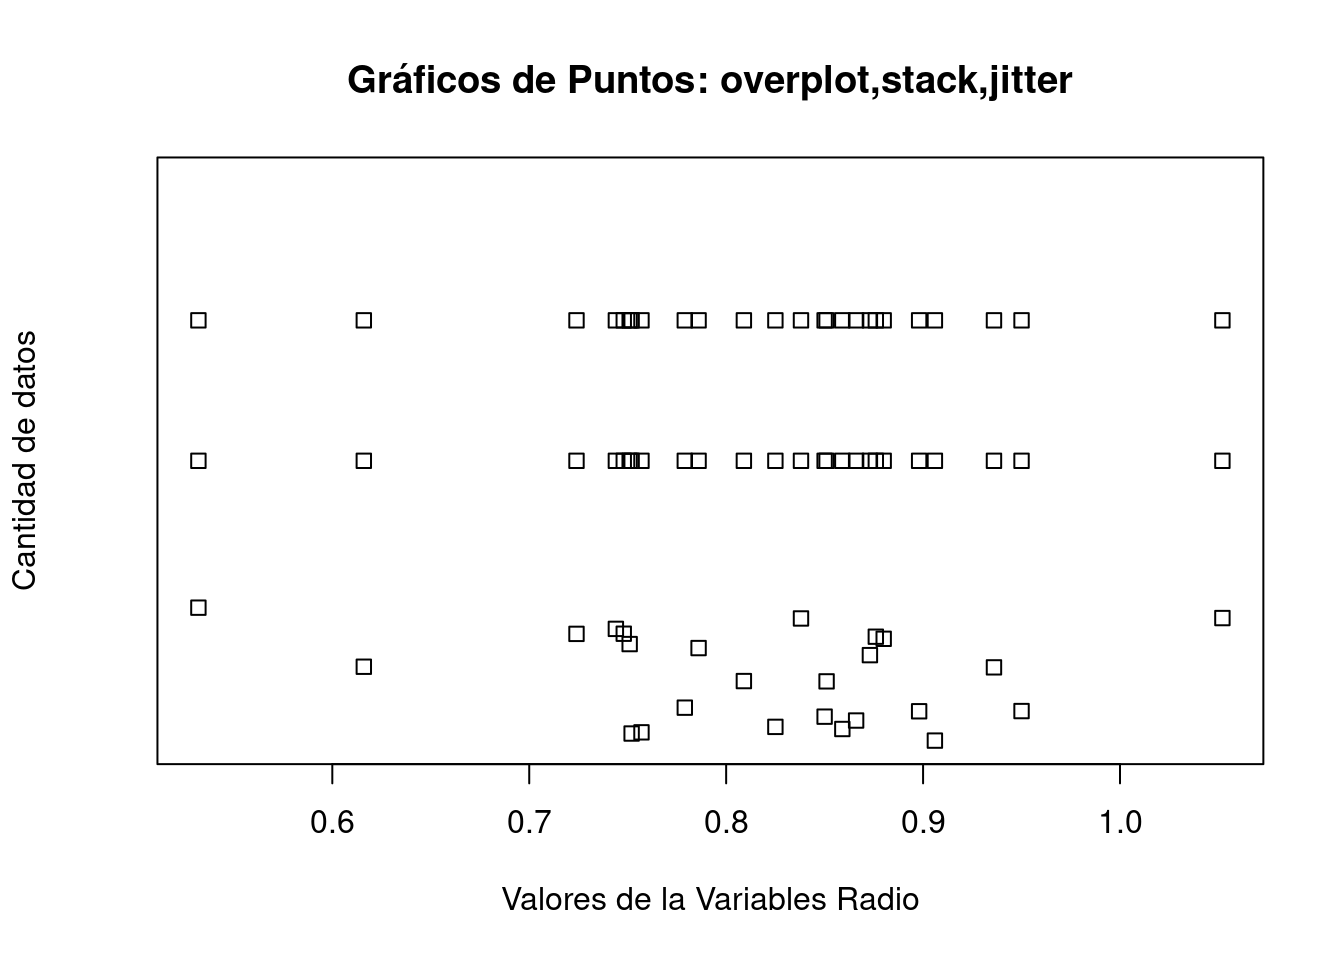
\includegraphics[width=0.8\linewidth]{figurasR/grafica1a-1} 

}

\caption{Gráficos de Puntos}\label{fig:grafica1a}
\end{figure}

\textbf{Gráficos de puntos para Datos Normales:}

\begin{figure}[H]

{\centering 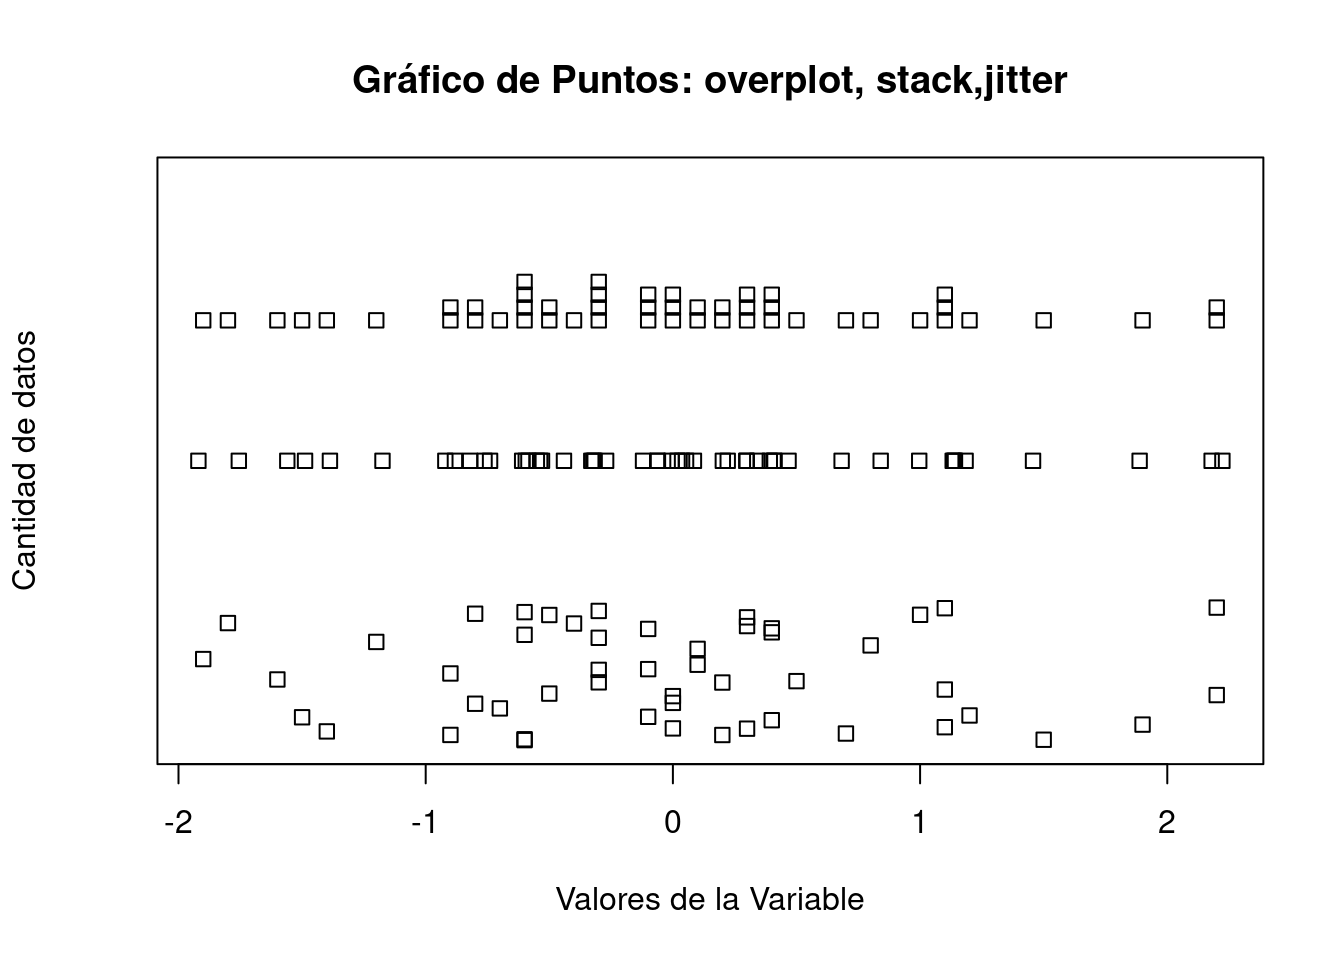
\includegraphics[width=0.8\linewidth]{figurasR/grafica1b-1} 

}

\caption{Gráficos de Puntos}\label{fig:grafica1b}
\end{figure}

\hypertarget{gruxe1ficos-de-dispersiuxf3n-o-scatterplot}{%
\subsection{Gráficos de Dispersión o
Scatterplot}\label{gruxe1ficos-de-dispersiuxf3n-o-scatterplot}}

\begin{figure}[H]

{\centering 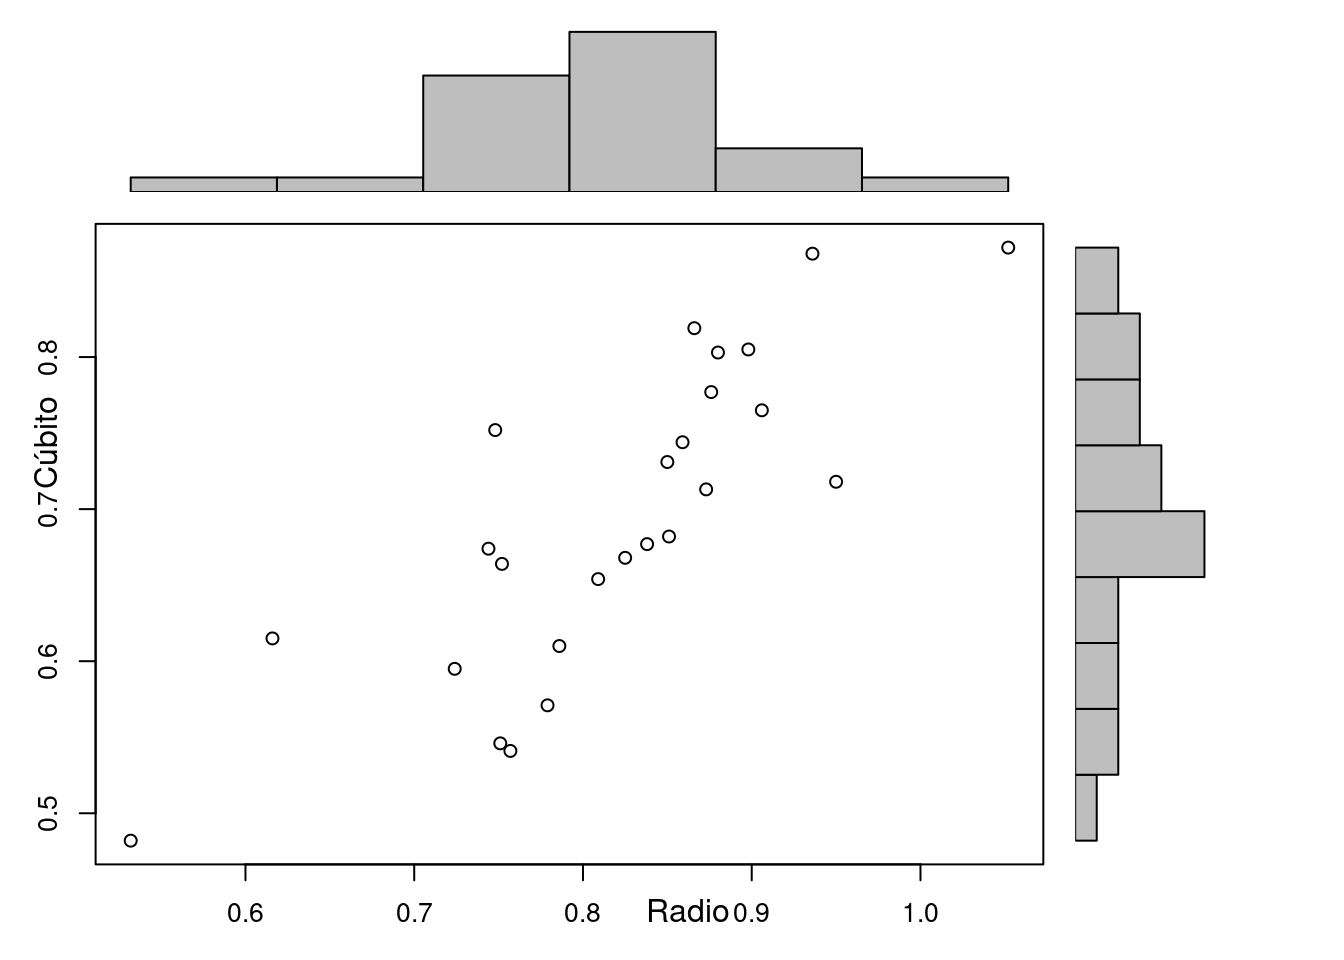
\includegraphics[width=0.8\linewidth]{figurasR/grafica1c-1} 

}

\caption{Gráficos de Dispersión con Histogramas}\label{fig:grafica1c}
\end{figure}

\begin{figure}[H]

{\centering 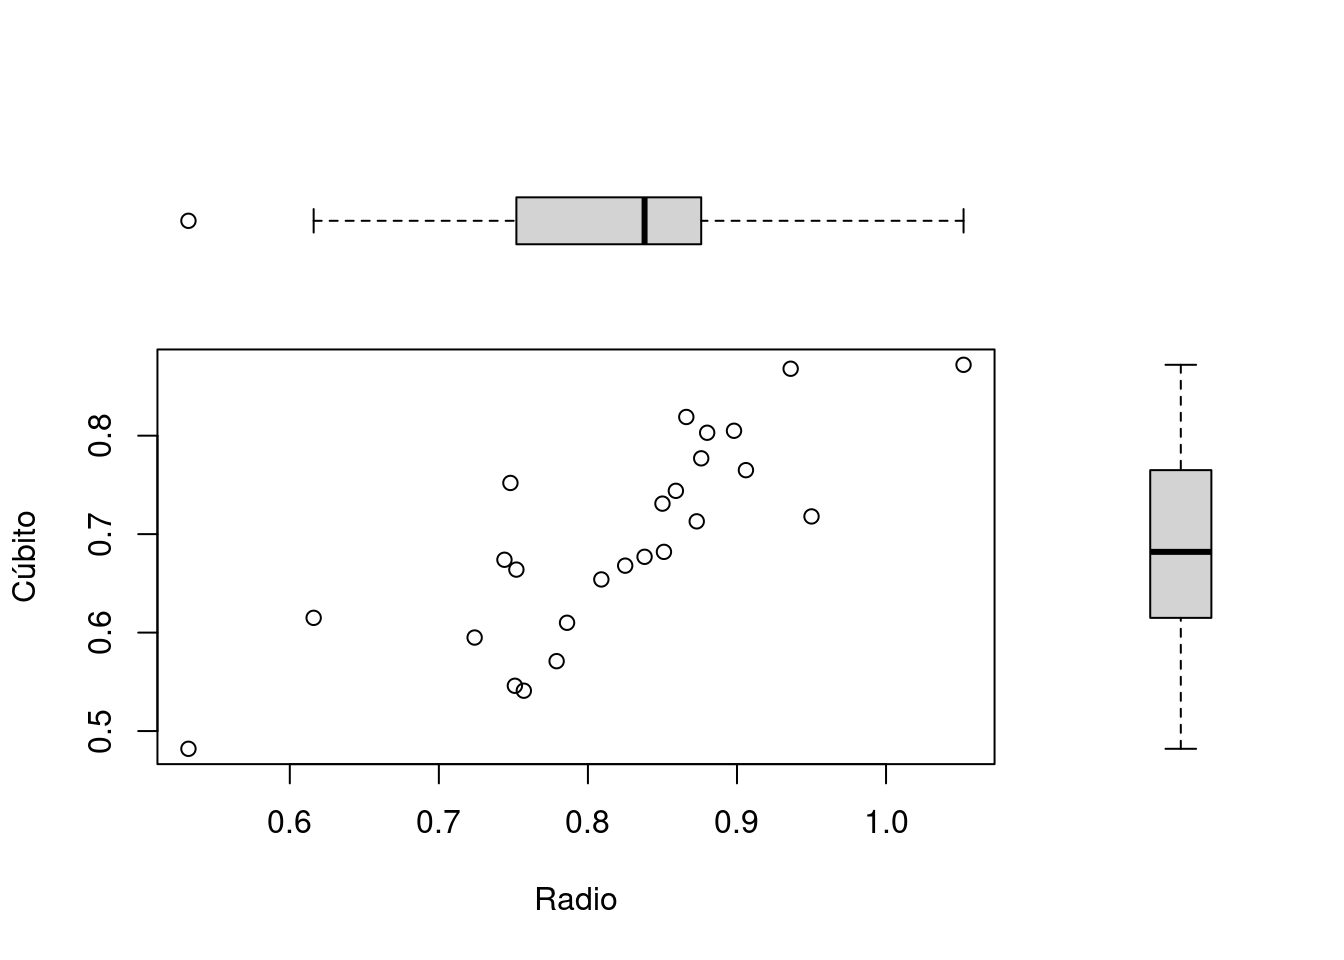
\includegraphics[width=0.8\linewidth]{figurasR/grafica1d-1} 

}

\caption{Gráficos de Dispersión con Box-Plot}\label{fig:grafica1d}
\end{figure}

\begin{figure}[H]

{\centering 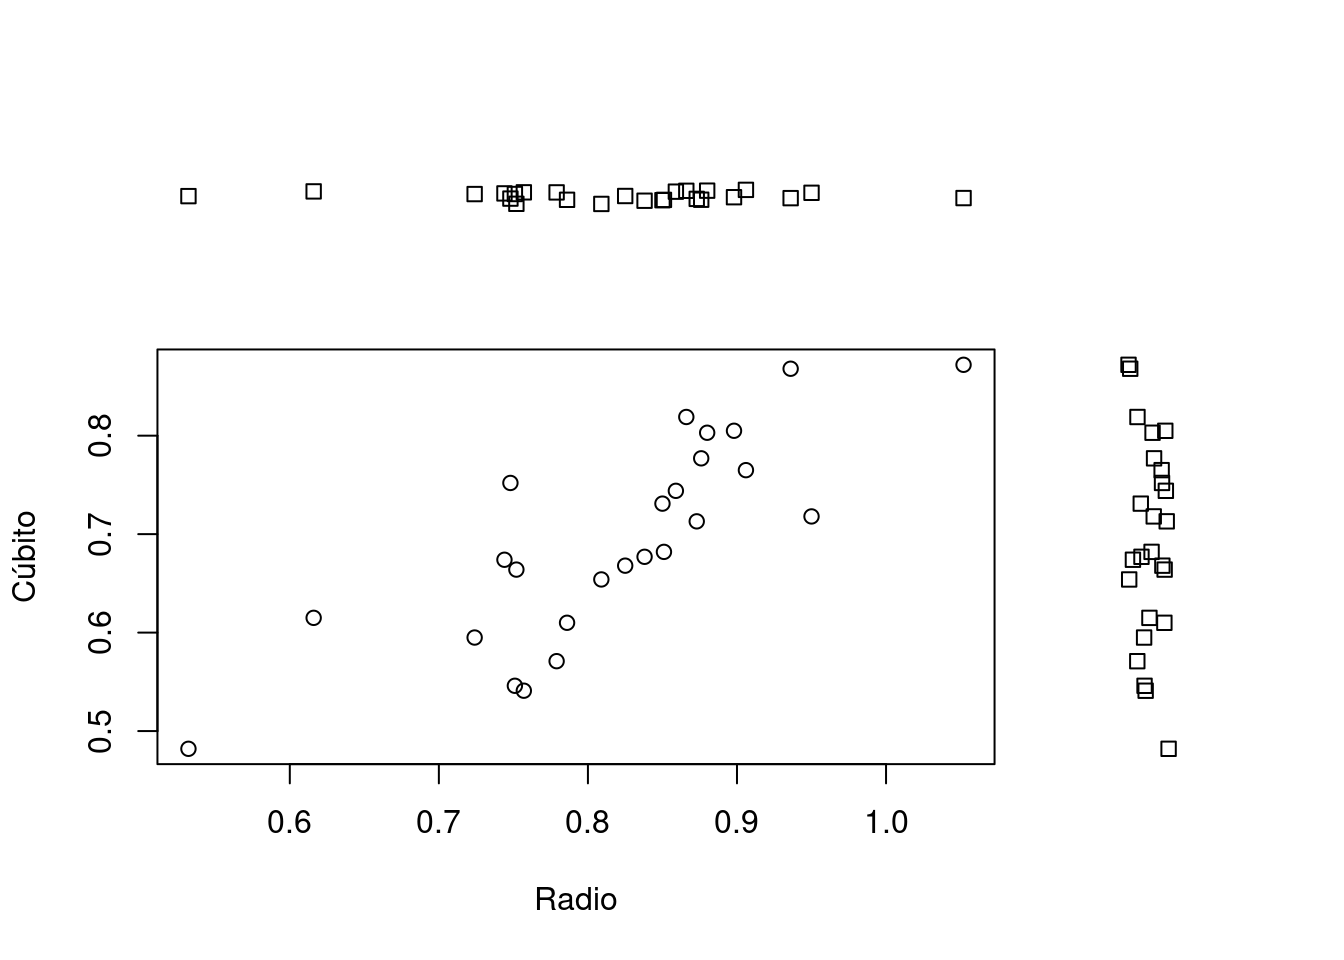
\includegraphics[width=0.8\linewidth]{figurasR/grafica1e-1} 

}

\caption{Gráficos de Dispersión con Gráficos de Puntos}\label{fig:grafica1e}
\end{figure}

\hypertarget{matriz-de-dispersiuxf3n}{%
\subsection{Matriz de Dispersión}\label{matriz-de-dispersiuxf3n}}

\begin{figure}[H]

{\centering 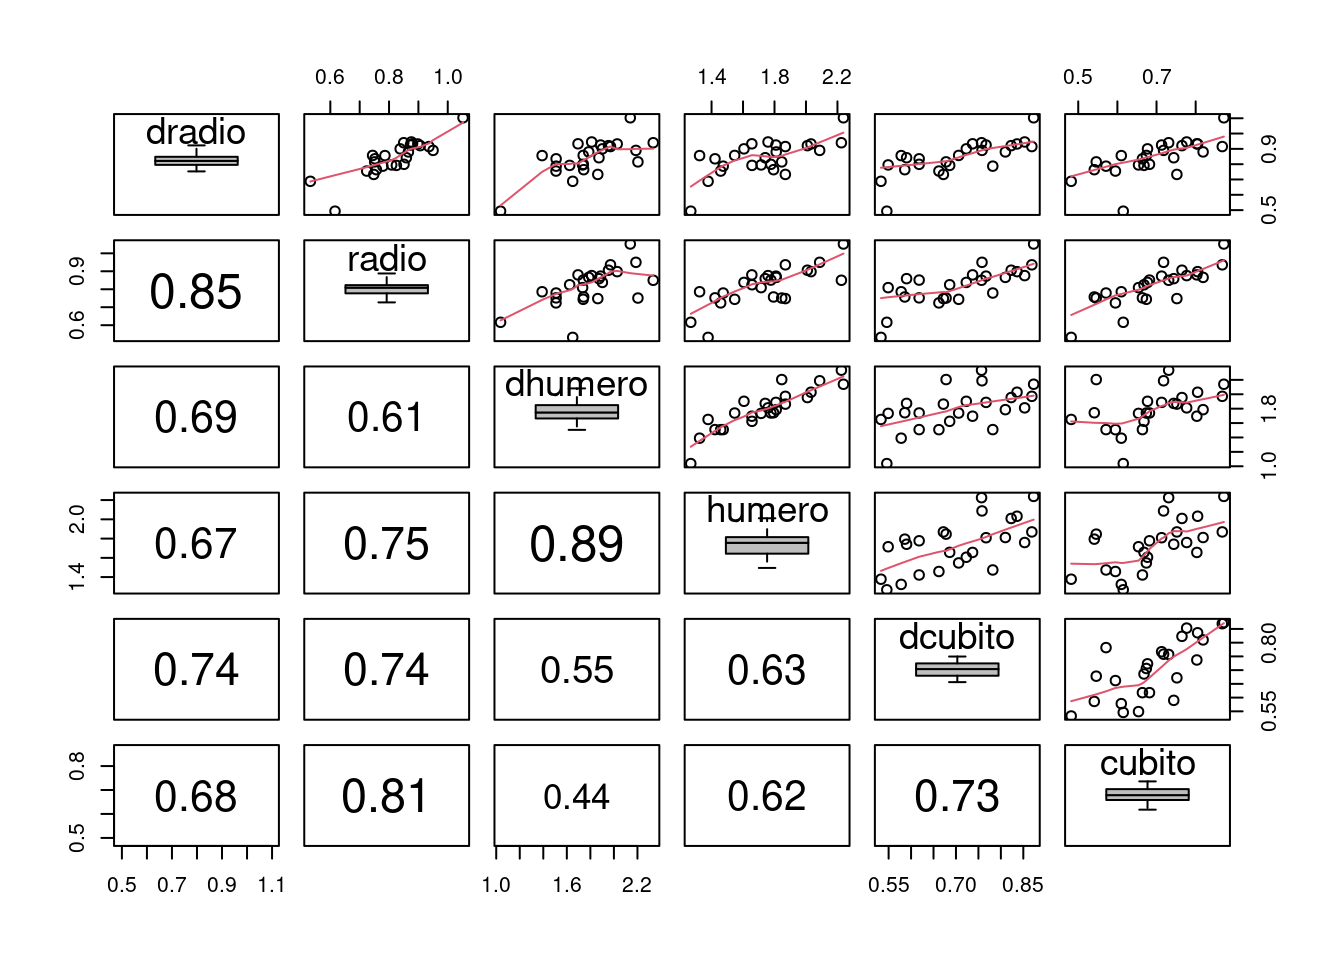
\includegraphics[width=0.7\linewidth]{figurasR/grafica1f-1} 

}

\caption{Matriz de Dispersión de Datos, Box-Plot-Corr}\label{fig:grafica1f}
\end{figure}

\begin{figure}[H]

{\centering 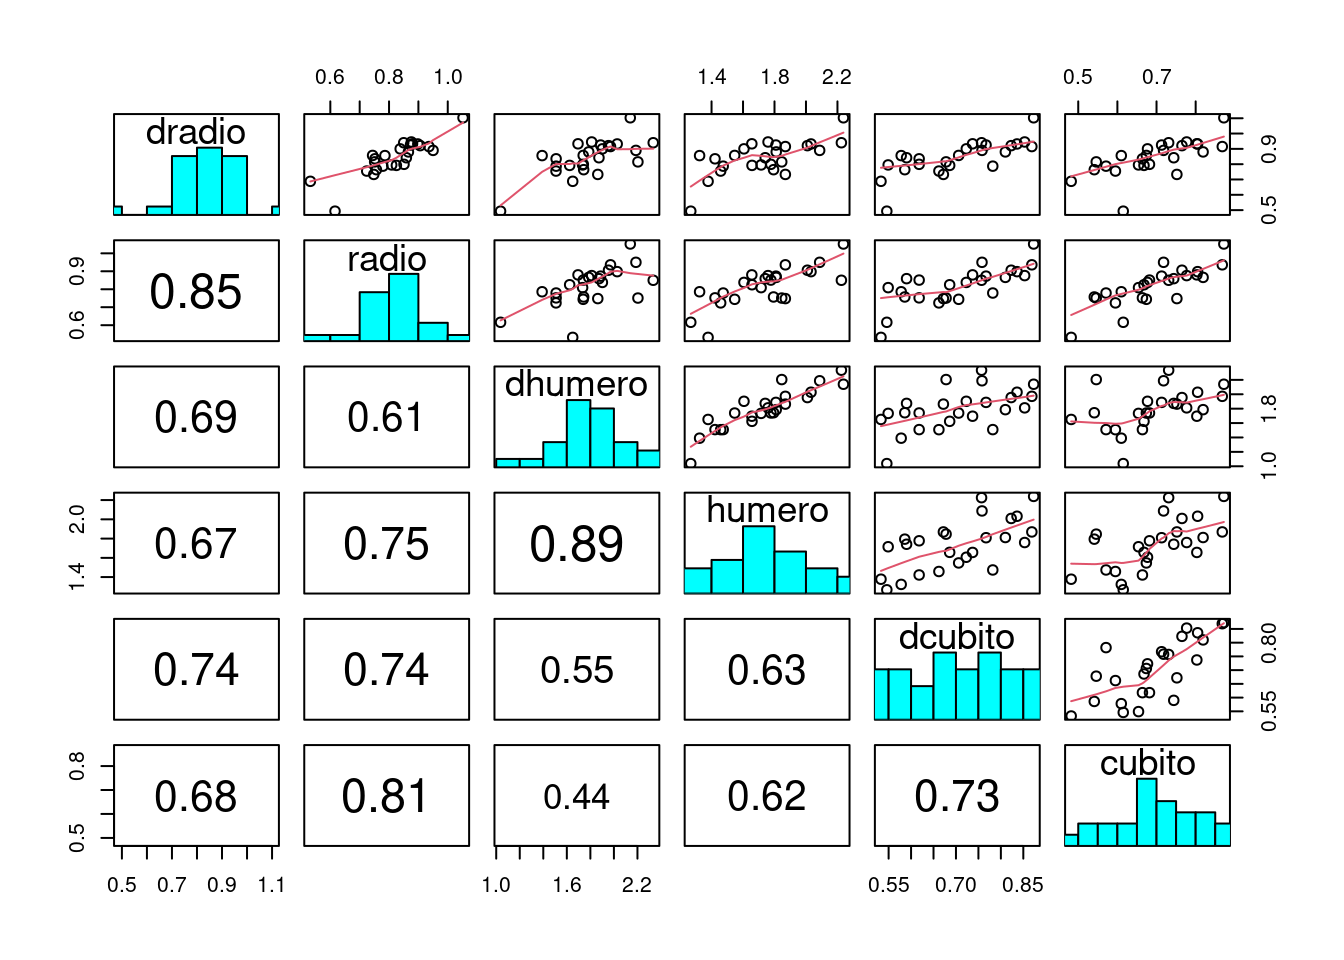
\includegraphics[width=0.7\linewidth]{figurasR/grafica1g-1} 

}

\caption{Matriz de Dispersión de Datos, Histogramas-Corr}\label{fig:grafica1g}
\end{figure}

\begin{figure}[H]

{\centering 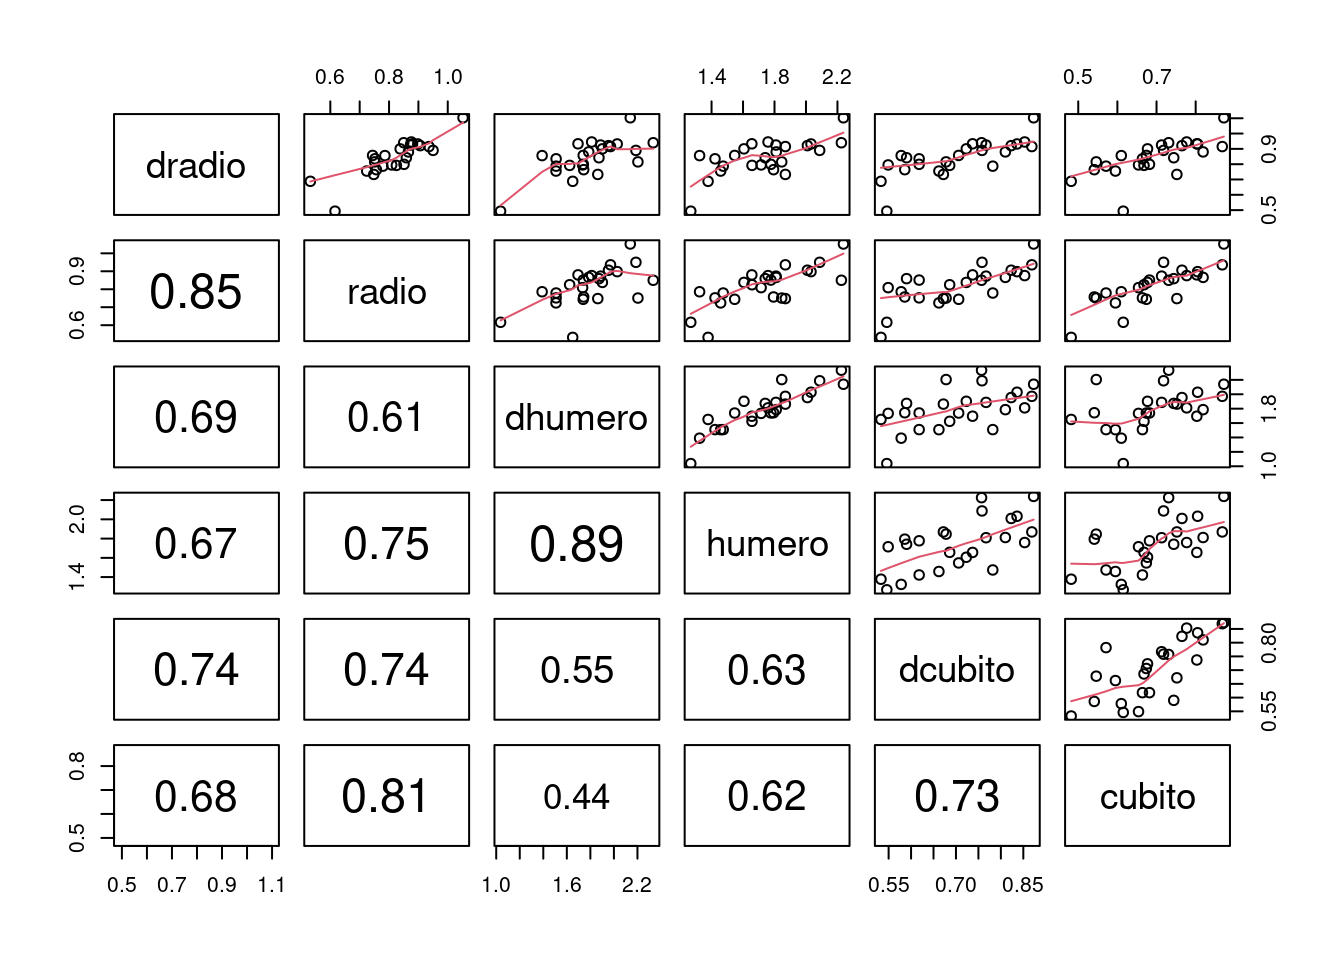
\includegraphics[width=0.7\linewidth]{figurasR/grafica1h-1} 

}

\caption{Matriz de Dispersión de Datos, Corr}\label{fig:grafica1h}
\end{figure}

\hypertarget{gruxe1fica-de-la-matriz-de-correlaciones}{%
\section{Gráfica de la Matriz de
Correlaciones}\label{gruxe1fica-de-la-matriz-de-correlaciones}}

\begin{figure}[H]

{\centering 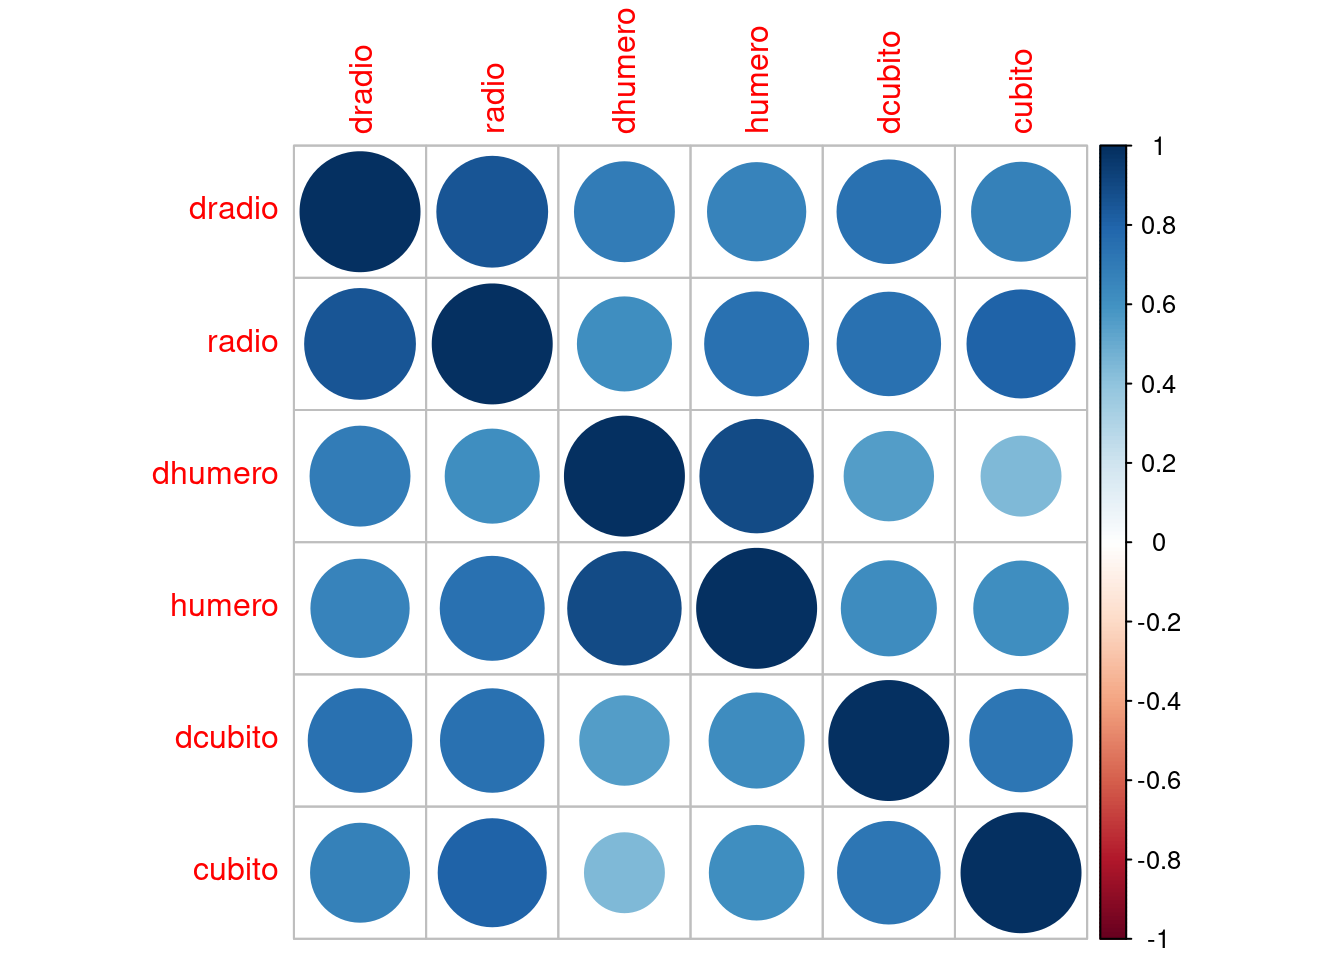
\includegraphics[width=0.6\linewidth]{figurasR/grafica1i-1} 

}

\caption{Matriz de Correlaciónes}\label{fig:grafica1i}
\end{figure}

\begin{figure}[H]

{\centering 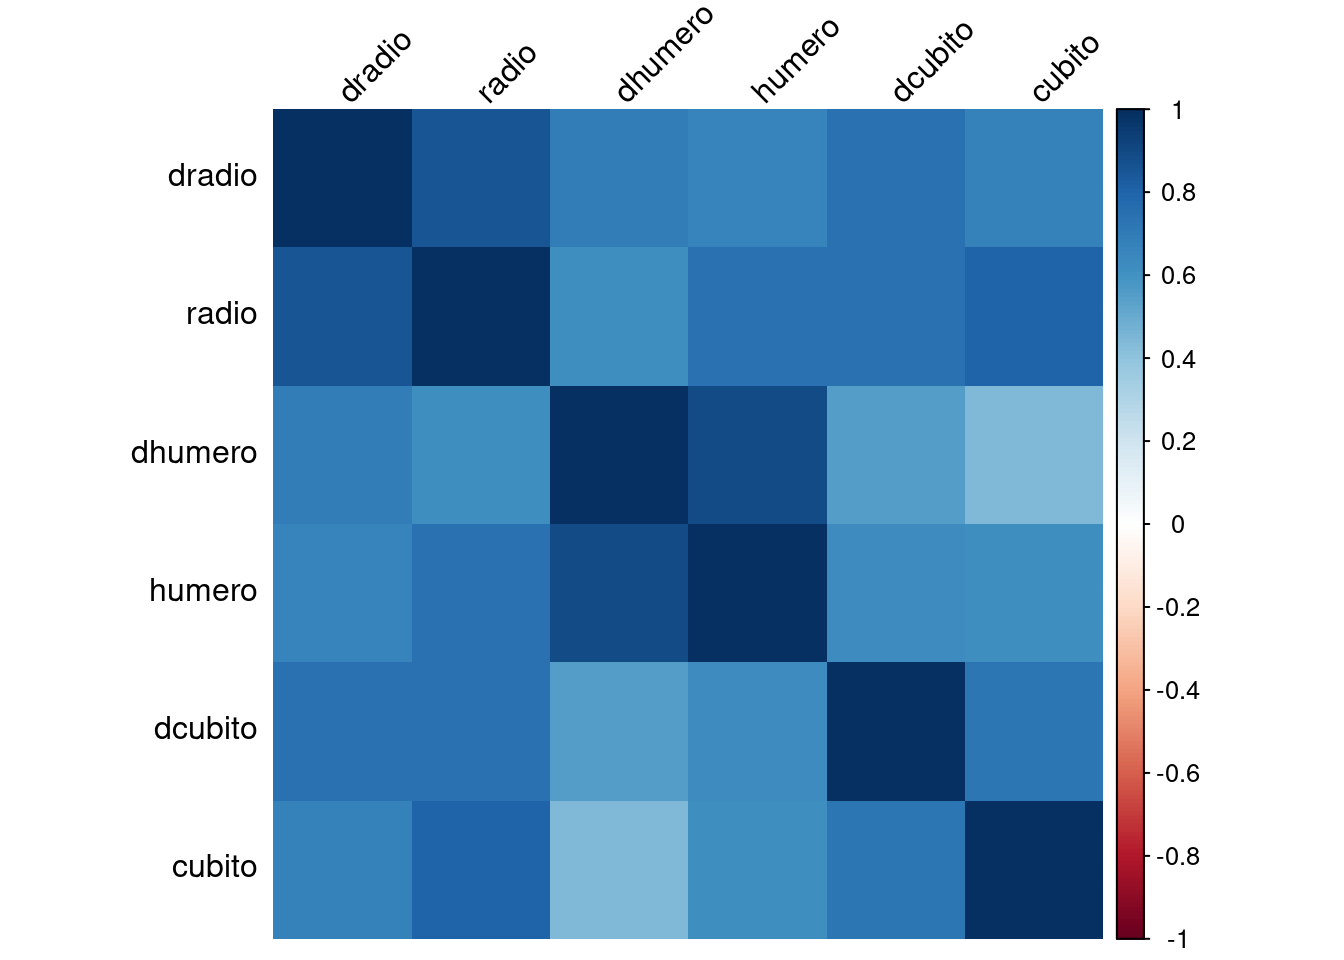
\includegraphics[width=0.6\linewidth]{figurasR/grafica1j-1} 

}

\caption{Matriz de Correlaciónes2}\label{fig:grafica1j}
\end{figure}

\begin{figure}[H]

{\centering 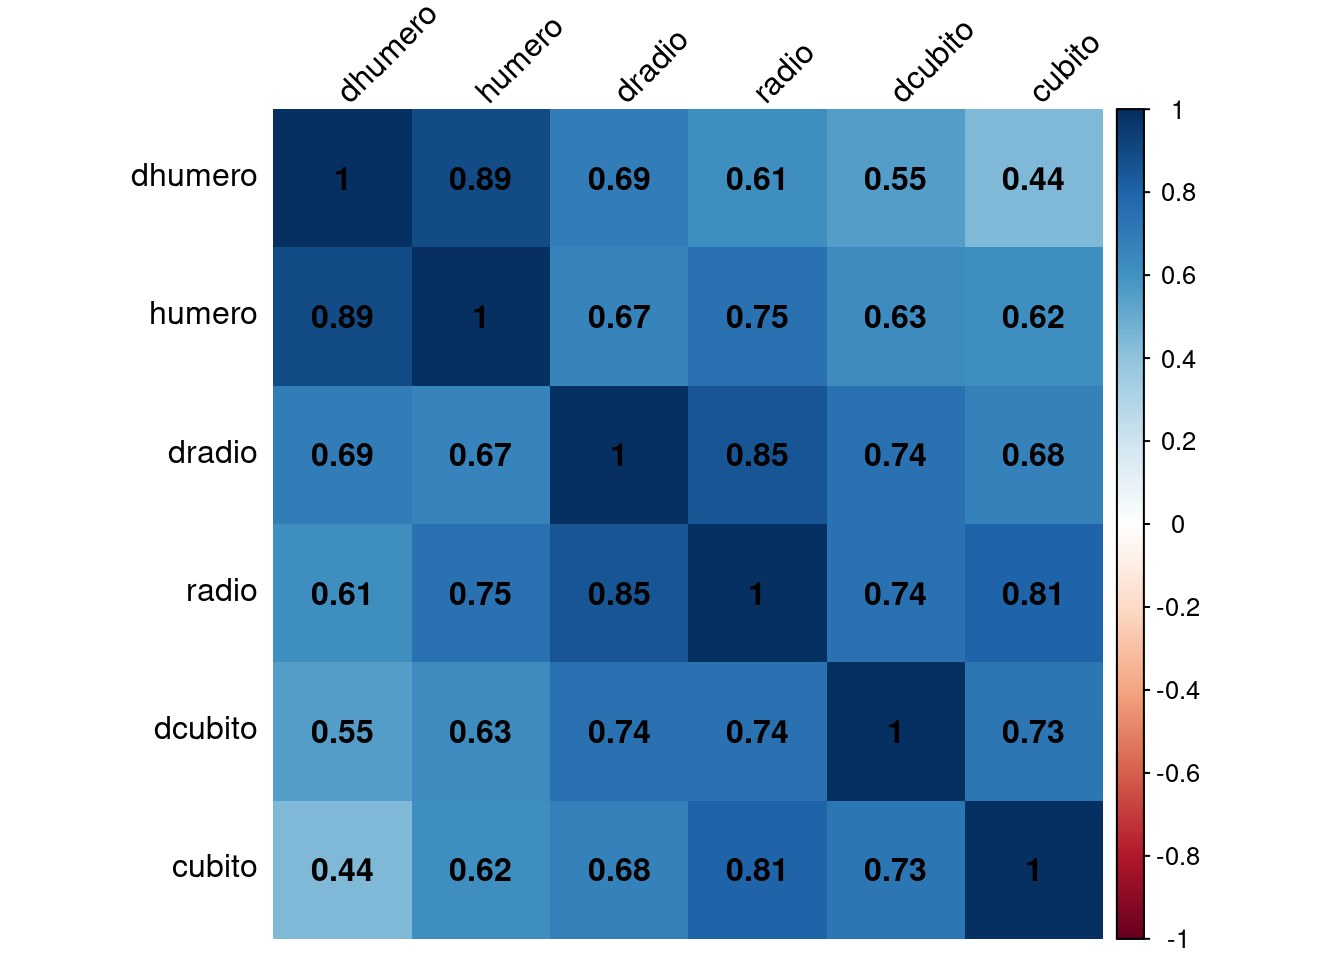
\includegraphics[width=0.6\linewidth]{figurasR/grafica1k-1} 

}

\caption{Matriz de Correlaciónes3}\label{fig:grafica1k}
\end{figure}

\begin{figure}[H]

{\centering 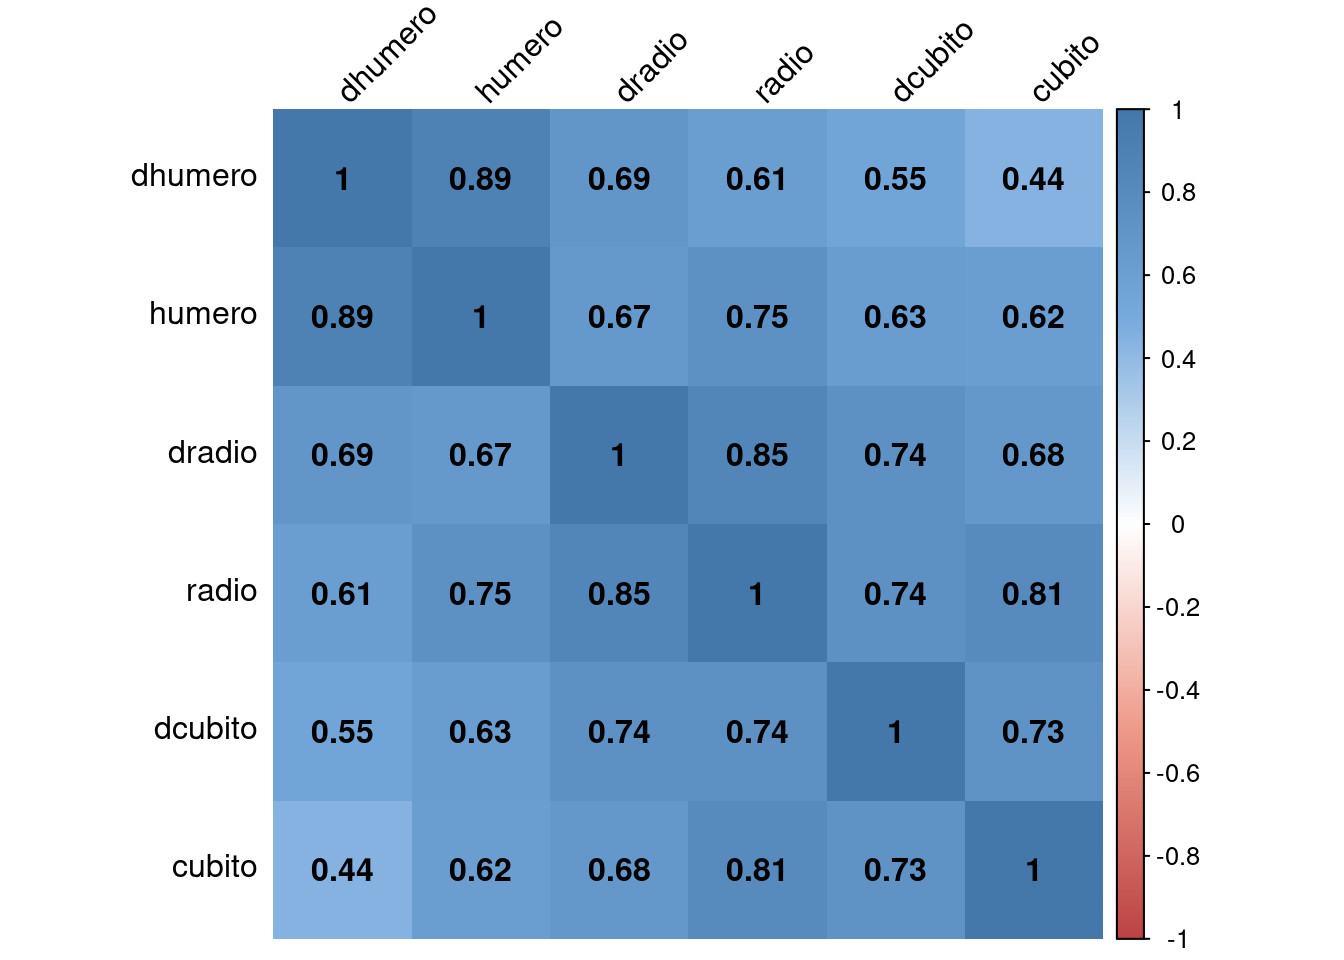
\includegraphics[width=0.6\linewidth]{figurasR/grafica1l-1} 

}

\caption{Matriz de Correlaciónes4}\label{fig:grafica1l}
\end{figure}

\begin{figure}[H]

{\centering 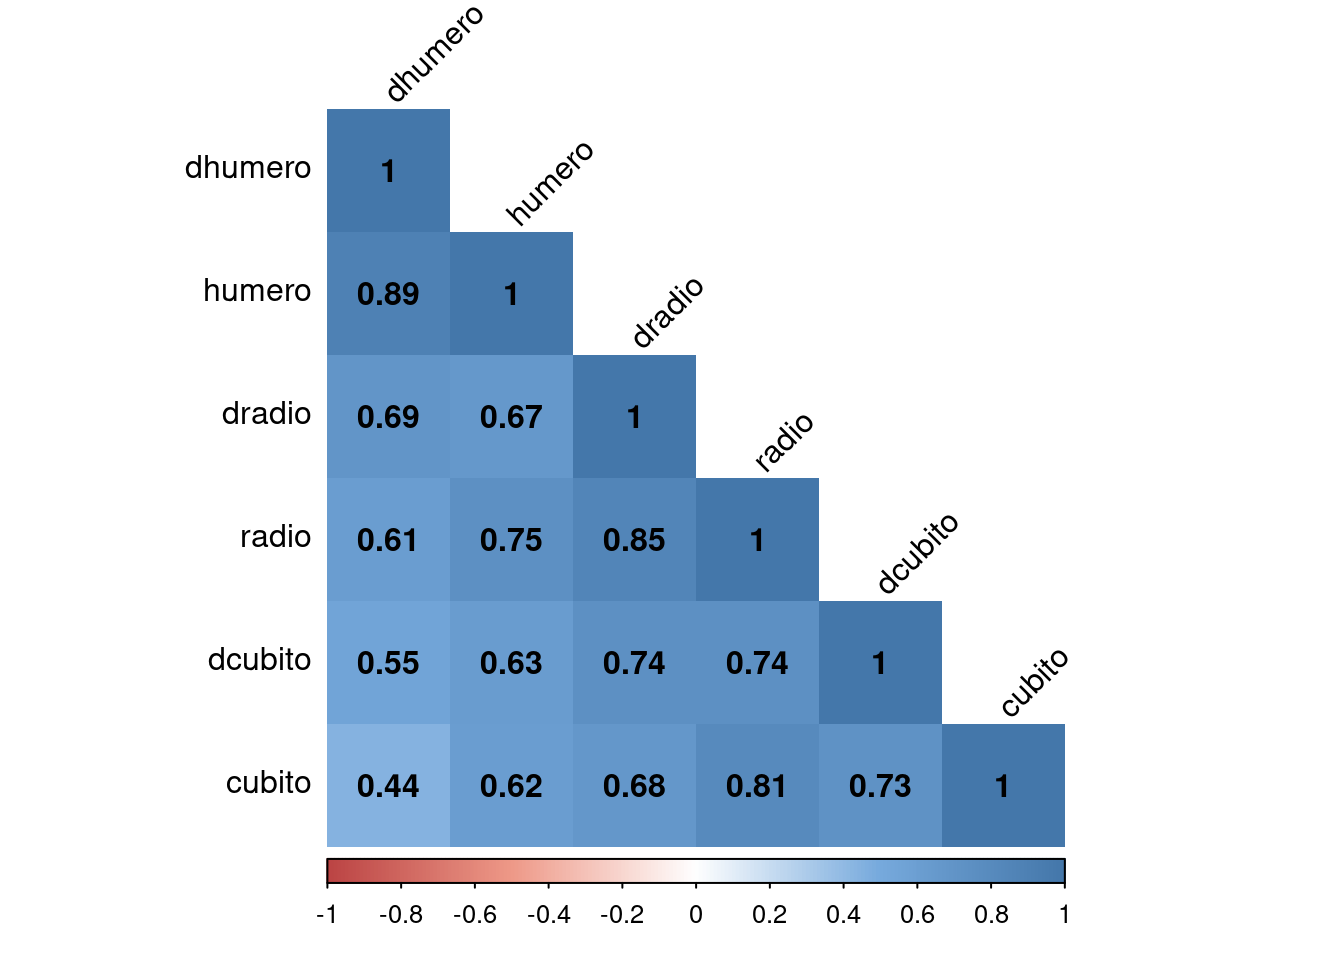
\includegraphics[width=0.6\linewidth]{figurasR/grafica1m-1} 

}

\caption{Matriz de Correlaciónes5}\label{fig:grafica1m}
\end{figure}

\begin{figure}[H]

{\centering 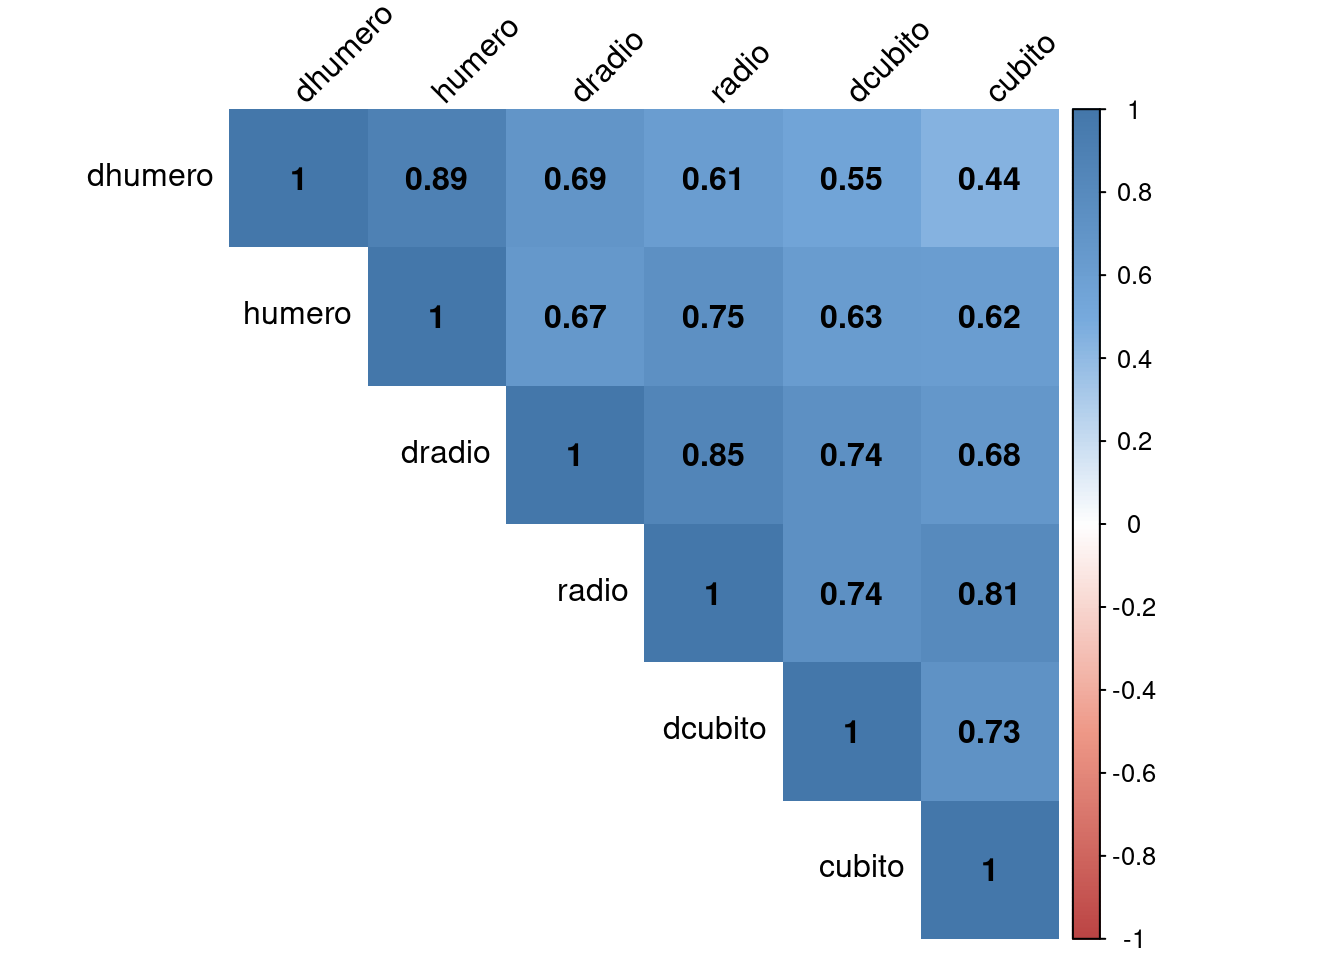
\includegraphics[width=0.6\linewidth]{figurasR/grafica1n-1} 

}

\caption{Matriz de Correlaciónes6}\label{fig:grafica1n}
\end{figure}

\begin{figure}[H]

{\centering 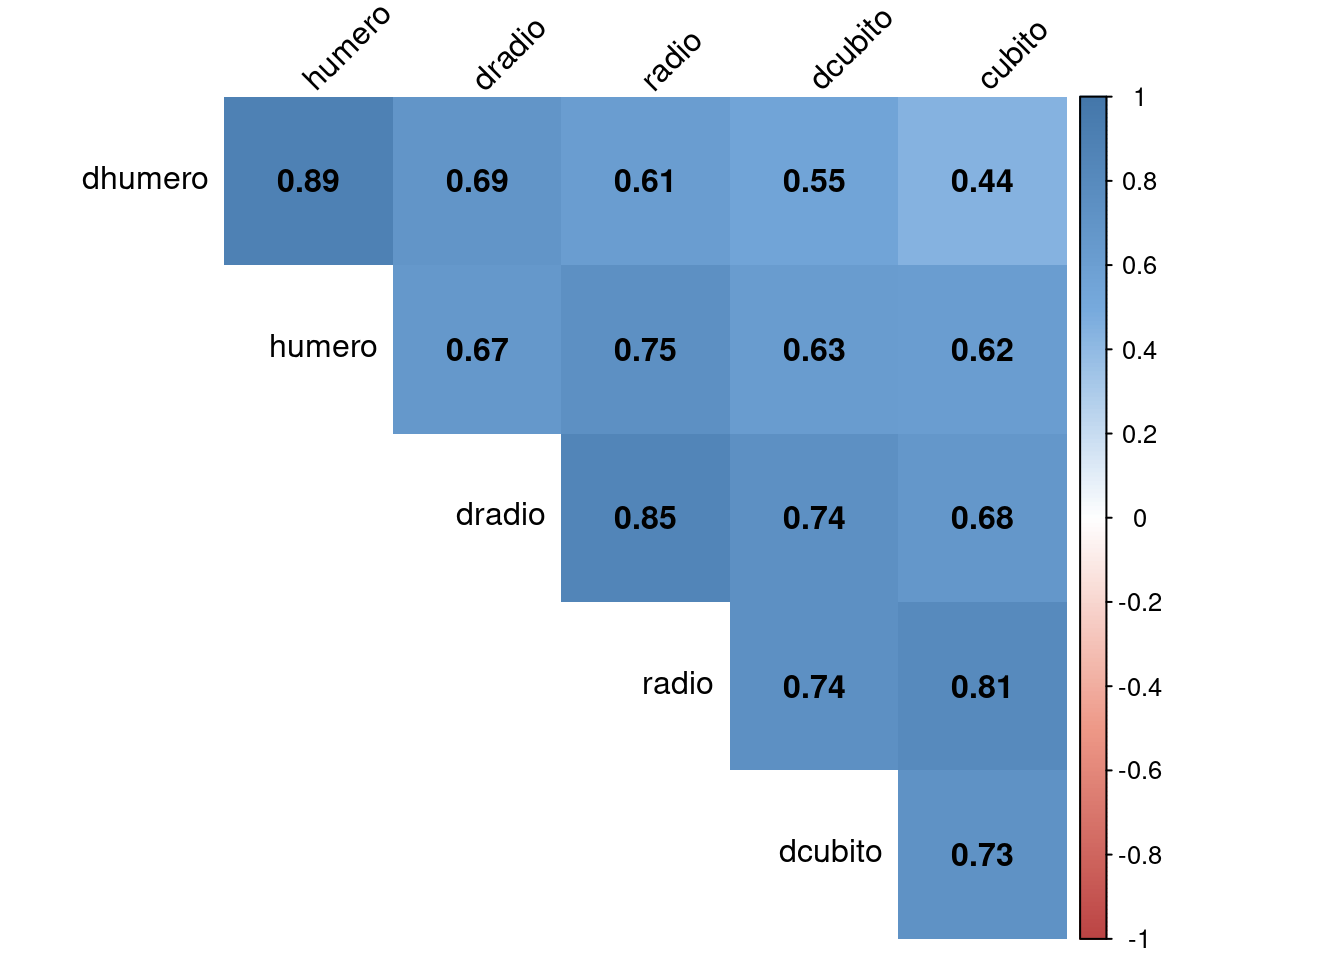
\includegraphics[width=0.6\linewidth]{figurasR/grafica1o-1} 

}

\caption{Matriz de Correlaciónes7}\label{fig:grafica1o}
\end{figure}

\begin{figure}[H]

{\centering 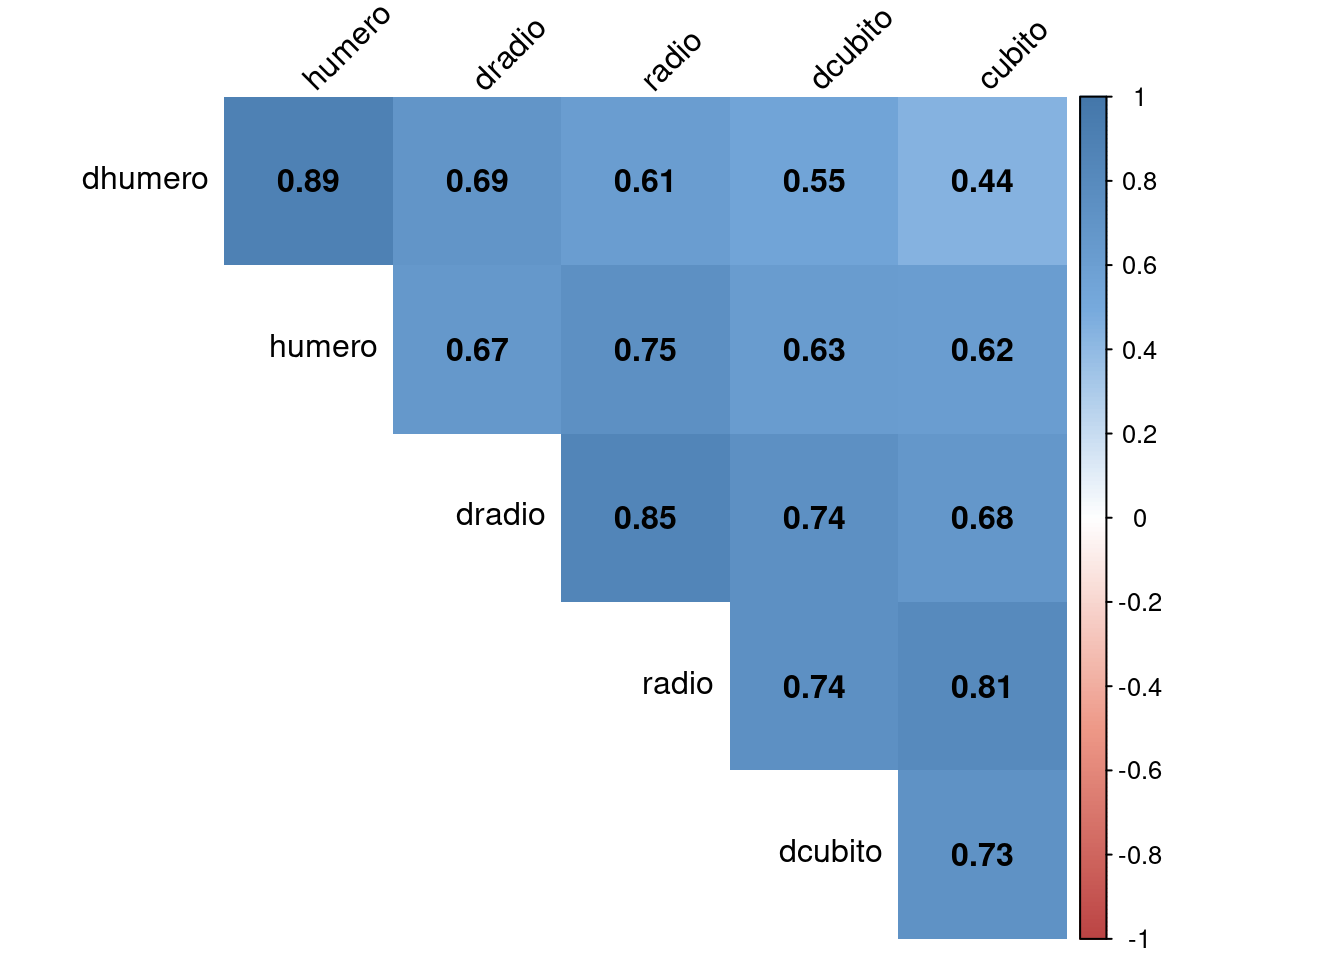
\includegraphics[width=0.6\linewidth]{figurasR/grafica1p-1} 

}

\caption{Matriz de Correlaciónes8}\label{fig:grafica1p}
\end{figure}

\begin{figure}[H]

{\centering 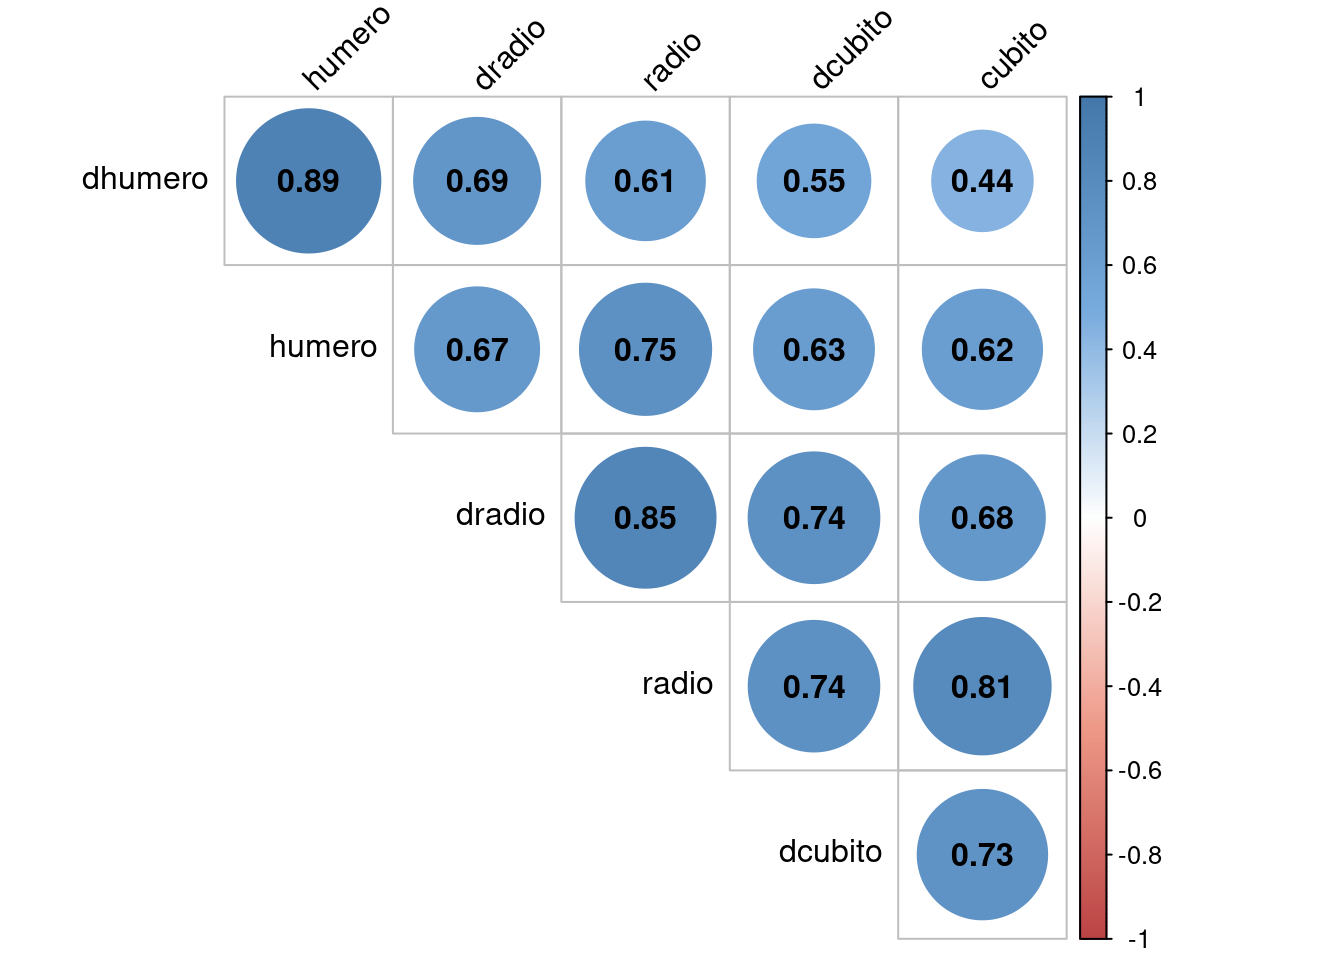
\includegraphics[width=0.6\linewidth]{figurasR/grafica1q-1} 

}

\caption{Matriz de Correlaciónes9}\label{fig:grafica1q}
\end{figure}

\begin{figure}[H]

{\centering 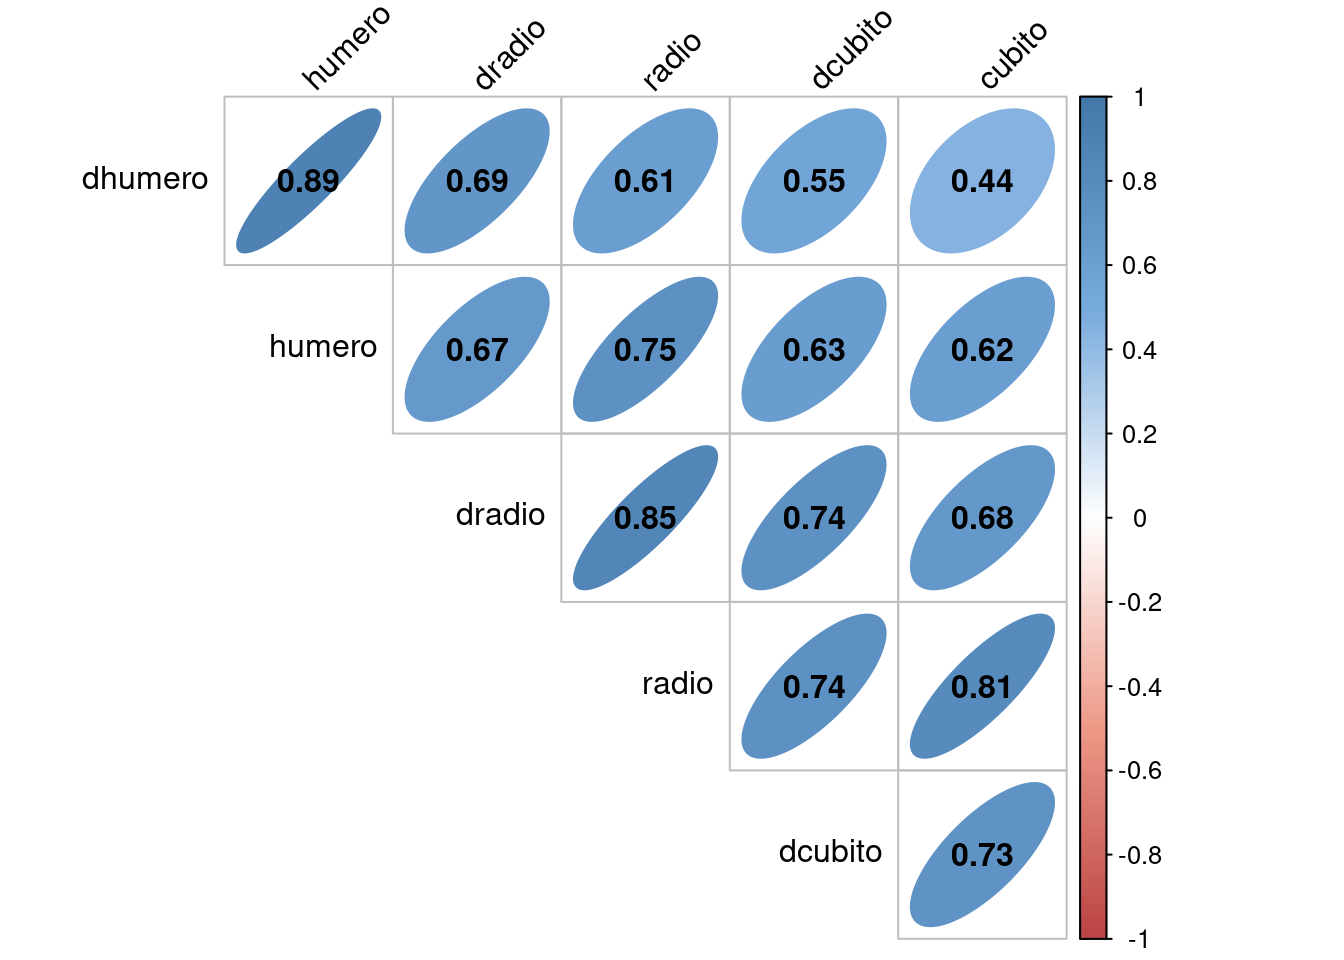
\includegraphics[width=0.6\linewidth]{figurasR/grafica1r-1} 

}

\caption{Matriz de Correlaciónes10}\label{fig:grafica1r}
\end{figure}

\begin{figure}[H]

{\centering 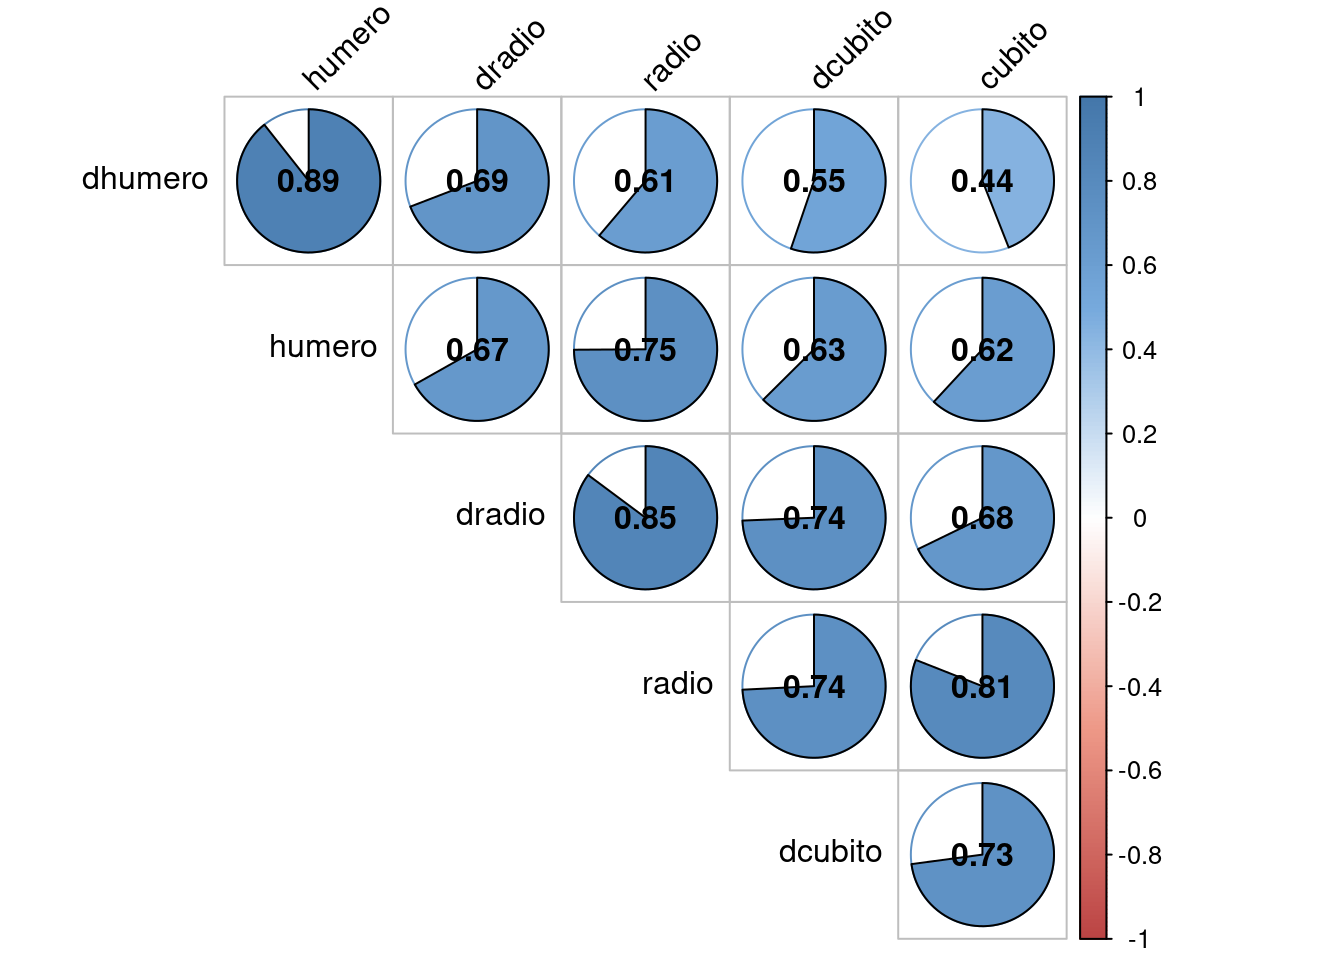
\includegraphics[width=0.6\linewidth]{figurasR/grafica1s-1} 

}

\caption{Matriz de Correlaciónes11}\label{fig:grafica1s}
\end{figure}

\begin{figure}[H]

{\centering 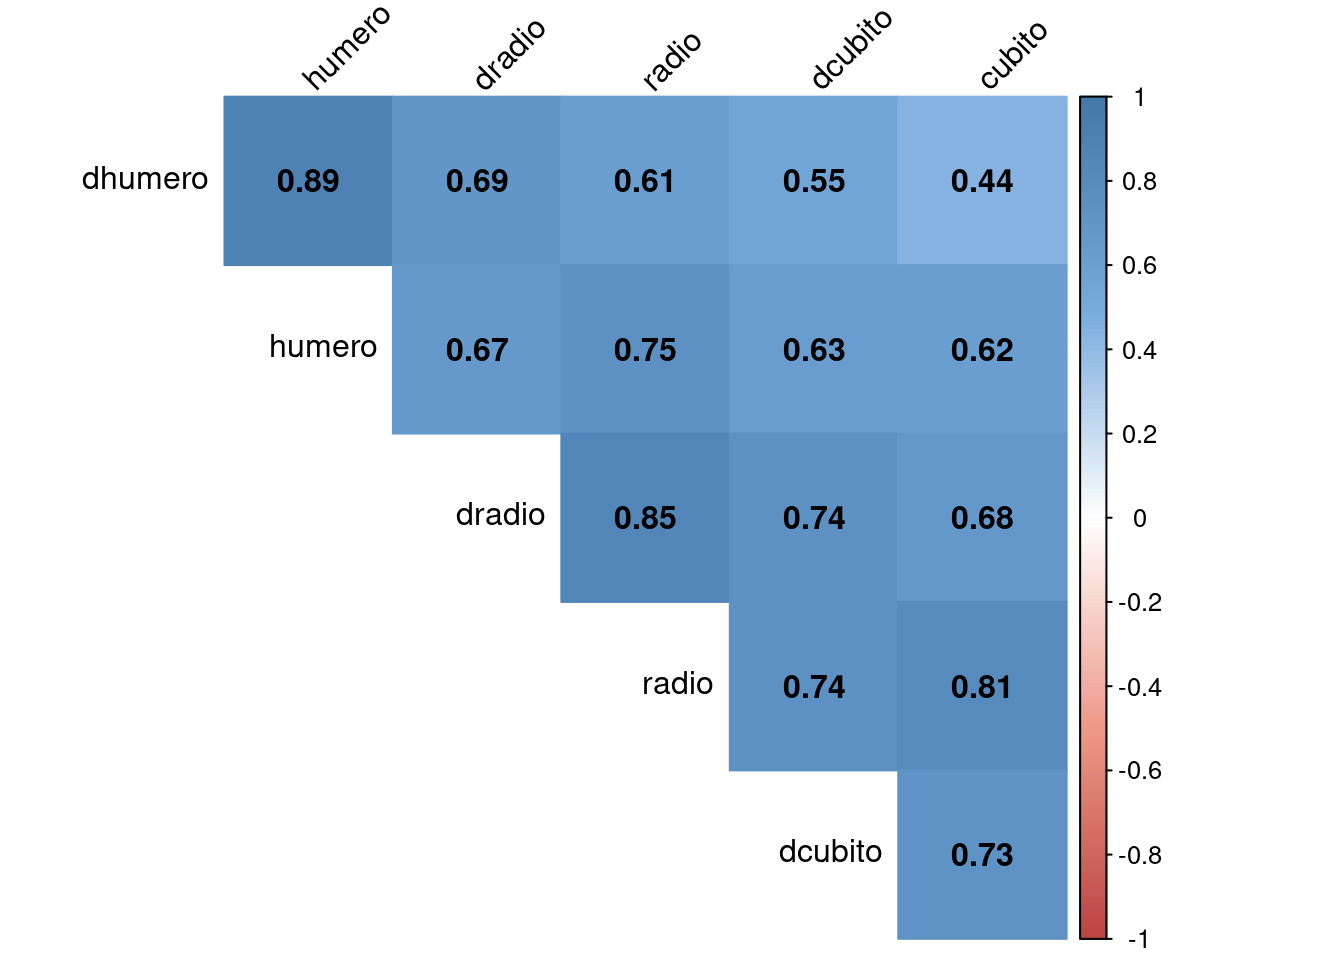
\includegraphics[width=0.6\linewidth]{figurasR/grafica1t-1} 

}

\caption{Matriz de Correlaciónes12}\label{fig:grafica1t}
\end{figure}

\begin{figure}[H]

{\centering 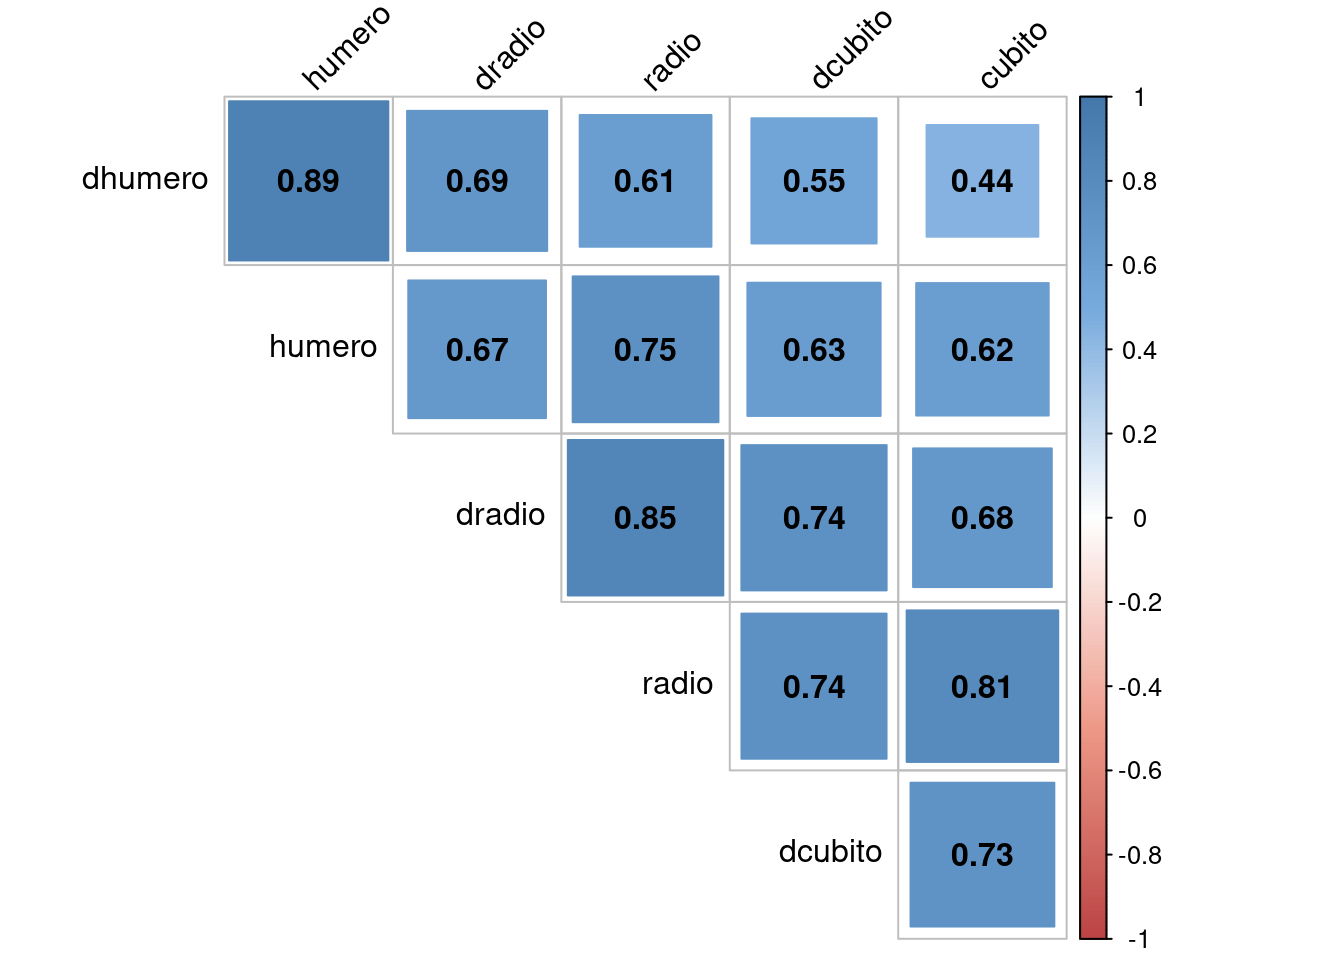
\includegraphics[width=0.6\linewidth]{figurasR/grafica1u-1} 

}

\caption{Matriz de Correlaciónes13}\label{fig:grafica1u}
\end{figure}

\begin{figure}[H]

{\centering 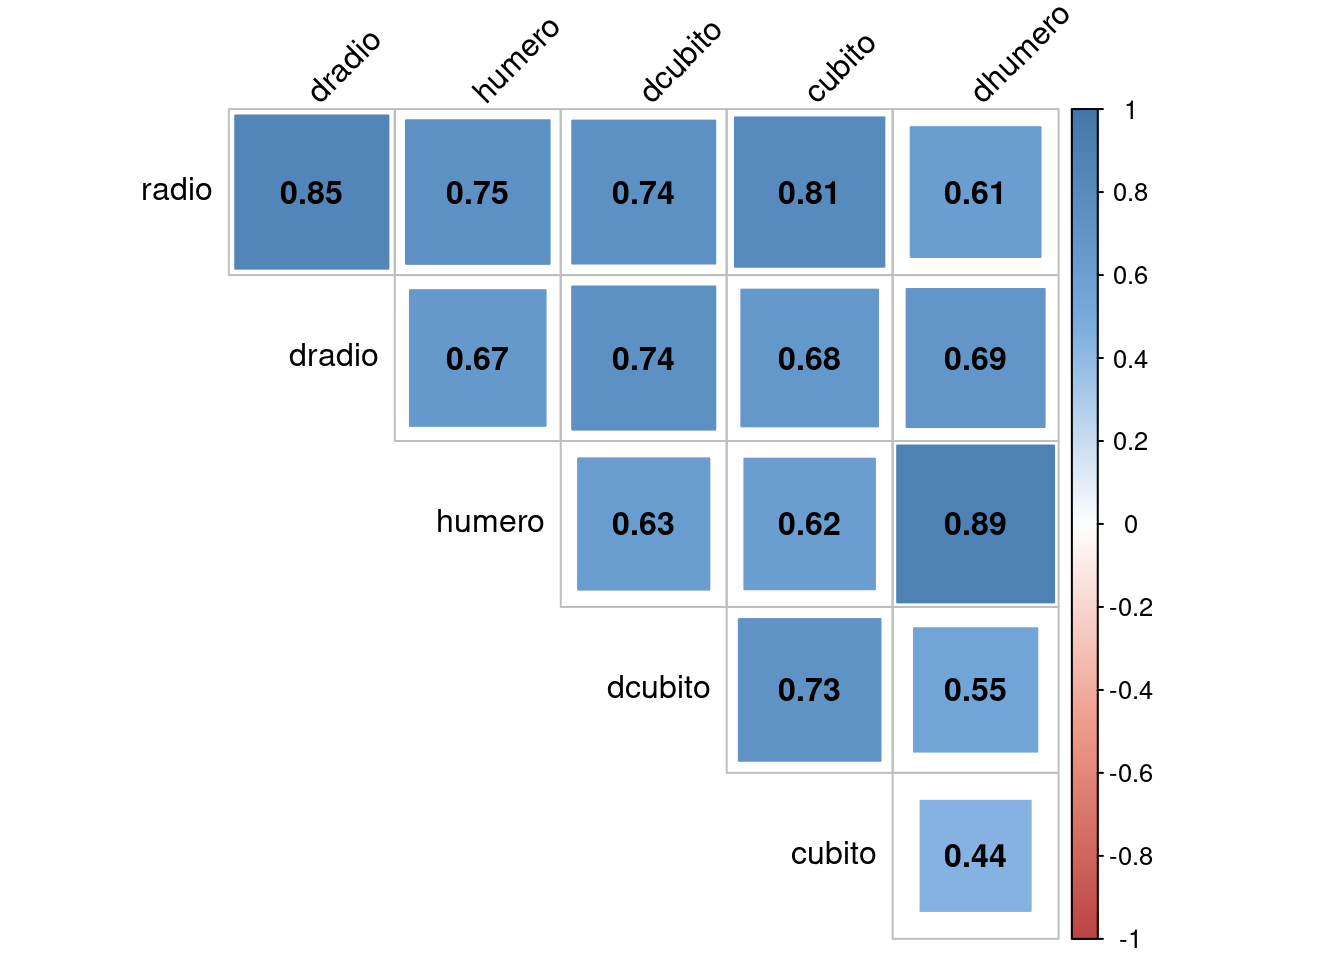
\includegraphics[width=0.6\linewidth]{figurasR/grafica1v-1} 

}

\caption{Matriz de Correlaciónes14}\label{fig:grafica1v}
\end{figure}

\begin{figure}[H]

{\centering 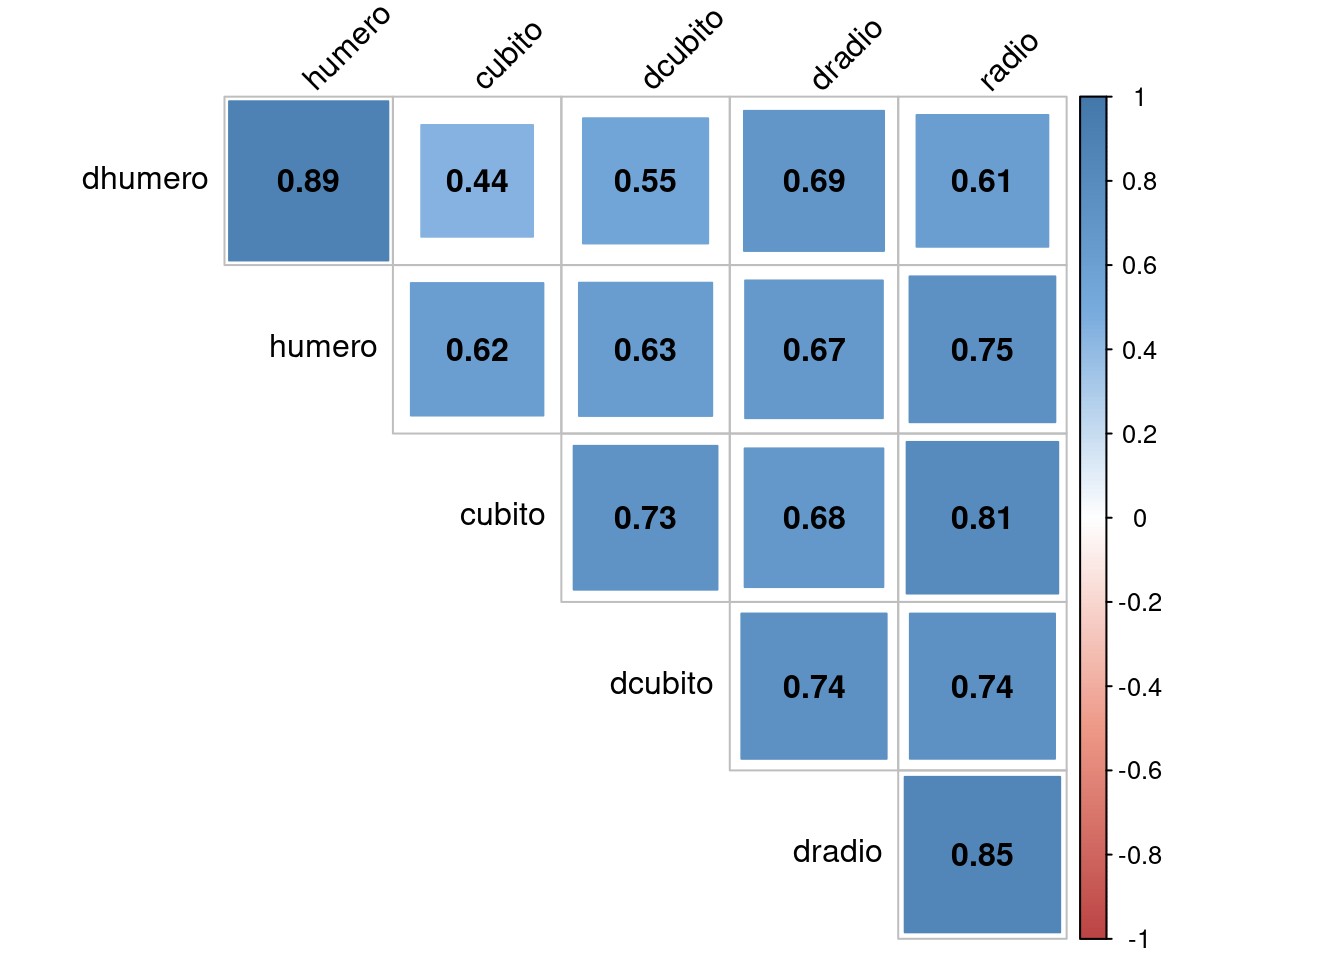
\includegraphics[width=0.6\linewidth]{figurasR/grafica1w-1} 

}

\caption{Matriz de Correlaciónes15}\label{fig:grafica1w}
\end{figure}

\bibliography{bib/library.bib,bib/paquetes.bib}


\addcontentsline{toc}{chapter}{Bibliografía}


\end{document}
